% Description of all calibrations

The two main purposes of the online software are the configuration for data taking and the online calibrations that are performed between runs for the calibration of the detector. There are a large number of different calibration tasks that need to be performed. This section contains a brief description of each calibration which may be run. For each calibration the following information is provided: the goal of the calibration, a step-by-step breakdown of what is being done, an example calib file and description of the parameters, an explanation of any output, pass/fail conditions, and the modification to the configuration as a result of the calibration. The next section, Sec.~\ref{sec:calibproc} describes when and in what order these calibrations are to be run, as well as how to analyze 'higher-level' processes which may consist of multiple iterations of different calibrations.

The calibrations described in this section are as follows. The AOHAndFEDChannelMappingTests checks whether the connections between AOH channels and FED channels are described properly in the configuration. The Delay25 calibration is used to ensure correct FEC communication. The ClockPhase calibration is used to adjust the timing of the signal digitization; a bad clock phase can also cause problems for most other calibrations.  The FEDBaselineCalibration is the most commonly used calibration; it sets the black level and provides an informative plot of the data buffer for each FED channel. The AOHBias and AOHGain calibrations further adjust the black levels. The ultrablack levels are adjusted for the TBM using the TBMUB calibration, and then the ROC UB levels are adjusted with the ROCUB calibration. The AddressLevels calibration is run in order to be able to decode pixel hits properly. The VcThrCalDel calibration adjusts the threshold and calibration injection delay. PixelAlive and SCurve calibrations test the efficiency of reading out an injected signal. More details are given below, along with descriptions of additional calibrations not included in the above list.

\subsection{AOHAndFEDChannelMappingTest}
\label{sec:AOHAndFEDChannelMappingTestCalibration}

\subsubsection{Introduction}
AOHAndFEDChannelMappingTest is not really a calibration, but rather a test to see whether the connections between AOH channels and FED channels in the configuration are correct.  The idea is to change the AOH bias for a single channel, and look to see whether the black level on the corresponding FED channel changes. This process is repeated for each channel. Those for which the black level changes are correctly connected; those for which there is no change are not connected correctly or have a mistake in the configuration files.

\subsubsection{Procedure}
The steps of this calibration are listed in order below.
\begin{enumerate}
\item Set the FED channels to the 2V peak-to-peak range in order to provide maximum dynamic range for the AOH bias scan.
\item Turn off the FED automatic baseline correction.
\item Set all FED optical receiver input offsets to 8, and channel offsets to 255.  These settings tend to put the signal in a range where the black level will not be stuck at the top or bottom of the range as AOH bias is varied.  (Maybe this step should be removed, and the default values should be used instead.)
\item Issue \verb|ClrCal| to all ROCs, and disable hits with the control register on all ROCs, to ensure that no hits are output.
\item Issue \verb|LRES| and \verb|CLRES| commands to all FEDs to clear the transparent data.  This ensures that no stale data is sitting in the buffer.
\item On the first channel, loop over AOH bias values.  On each trigger, inspect the transparent buffer and look for the start of the signal.  Record the black levels in the time slots preceeding the start of the signal.  Keep track of the mean black level and the standard deviation for each AOH bias value.  A plot of this scan is written to a ROOT file.
\item Inspect the scan of black level vs.~AOH bias.  If the black level varies as AOH bias changes, this channel is properly connected.  If the black level is constant, this channel is flagged as improperly connected.  (Quantitatively, the $\chi^2$ of the scan data is evaluated for the hypothesis of a flat line.  If $\chi^2/\mathrm{d.o.f.} > 100$, the scan data is considered to vary; otherwise it is considered constant.)  One exception is if the scan is constant at the top or bottom of the range (1023 or 0).  In this case the signal is out of range, and so the connectivity test is inconclusive.
\item Set AOH bias back to the default value (from the configuration).  This ensures that channels are not falsely flagged as being stuck at the top of the range.  If, say, two FED channels were swapped in the configuration, the first one scanned would show up as incorrectly connected.  With the AOH left at the highest scan point, when the FED channel that is actually connected to that AOH is checked later, the black level will appear to be stuck at the top of the range.  Setting that AOH back to its default value should put the black level on that channel back into the middle of the range.
\item Repeat the AOH bias scan for each channel in the configuration.
\item Print a summary to the screen.  Thus summary gives the number of channels which are properly connected, improperly connected, or for which the test was inconclusive.  Improperly connected and inconclusive channels are then listed.
\end{enumerate}

\subsubsection{Parameters}
An example calib.dat file for the AOHAndFEDChannelMappingTest is given below.

\begin{verbatim}
Mode:  AOHAndFEDChannelMappingTest
Parameters:
ScanMin        0
ScanMax        50
ScanStepSize   5
printFEDRawData         no
printScan               no
Rows:
Cols:
VcalHigh
Repeat: 10
ToCalibrate:
all
\end{verbatim}

A number of parameters in \verb|calib.dat| may be used to control the test. The ``\verb|Repeat:|" parameter determines the number of triggers at each AOH bias scan point.  The ``\verb|ToCalibrate:|'' parameter is used to determine which channels are calibrated.  Note that the rows, columns, and DAC scan settings in \verb|calib.dat| are completely ignored. Some optional parameters may also be set.  All have default values which will be used if the parameter is not set.  These parameters, their defaults, and their functionality are given in Table~\ref{tab:AOHAndFEDChannelMappingTestParameters}.

\begin{table}
\centering
\caption{Optional parameters for AOH and FED channel mapping test.}
\label{tab:AOHAndFEDChannelMappingTestParameters}
\begin{tabular}{l@{~~~~}r@{~~~~}l}
\hline
\hline
Parameter & Default & Description \\
\hline
ScanMin                     &   0 & Low end of AOH bias scan range \\
ScanMax                     &  50 & High end of AOH bias scan range \\
ScanStepSize                &   5 & Step size for AOH bias scan \\
printFEDRawData             &  no & Whether to print decoded transparent buffer \\
printScan                   &  no & Whether to print the AOH bias scan to the screen \\
\hline
\hline
\end{tabular}
\end{table}

\subsubsection{Output}
A summmary of the number of channels which are properly connected, improperly connected, or inconclusive is printed to the screen and may be seen in the PixelSupervisor logfile.  In addition, the names of the channels which are improperly connected or inconclusive are given.  The calibration succeeds if all channels are properly connected.

\subsubsection{Results}
This calibration does not produce any new configuration settings.  Any mistakes in the AOH and FED channel mapping revealed by the calibration must be adjusted manually. 

\subsection{ClockPhaseCalibration}
\label{sec:ClockPhaseCalibration}

\subsubsection{Introduction}
The FED has a delay (0 to 15) that goes in steps of 25/16 ns. In addition to the delay there is a phase that controls when the data is latched. Certain combinations of the delay and phase are invalid and result in garbage ADC values. This calibration adjusts the delay such that the FED signal is sampled at the transition from black to ultrablack in the TBM trailer.  An older version of the calibration, where the delay is set such that the FED signal is sampled at stationary points of the signal. 

A detailed description of this algorithm is presented in Appendix~\ref{sect:phaseanddelay}.

\subsubsection{Procedure}
 In this calibration the 32 values of the phase and delay (16 delay, 2 phase) are scanned. For each setting of the phase and delay a fixed number of events (typically around 10) is read out in transparent mode. The FED signal over 100 clocks is stored for each event. The signals for the multiple events are used to construct a single signal with noise estimate. The signal is purged (ADC value set to 0 for settings which are known to give garbage ADC values), ordered (ADC values for given delay values within a clock are rotated to give a continuous signal), and shifted such that the signals for phase 0 and phase 1 overlap. The phase 0 and phase 1 signals are then averaged. This final signal is then analyzed to determine the optimal delay setting.  Currently the delay is chosen for which the FED signal is sampled closest to the point where the transition from black to ultrablack occurs in the TBM trailer. In an older version of the calibration, the delay is chosen such that the signal is sampled at stationary points.

\subsubsection{Parameters}

An example of a \verb|calib.dat| file for the ClockPhaseCalibration is given below.

\begin{verbatim}
Mode: ClockPhaseCalibration
Rows:
Cols:
Vcal:
100 100 5
Repeat:
10
ToCalibrate:
all
\end{verbatim}

A number of parameters in \verb|calib.dat| may be used to control the test. The ``\verb|Repeat:|" parameter determines the number of triggers at each scan point.  The ``\verb|ToCalibrate:|'' parameter is used to determine which channels are calibrated.  The ``\verb|Vcal:|'' parameter sets the charge injected when running the calibration. In addition, as described in Appendix~\ref{sect:phaseanddelay} one can change the algorithm used to find the best phase and delay with an optional parameter.  To do this, the following lines would be added to \verb|calib.dat|:

\begin{verbatim}
Parameters:
oldMode Yes
\end{verbatim}

\subsubsection{Output}
This calibration writes results to an output ROOT file. For each channel there are four output canvases:
\begin{verbatim}
PhaseAndDelayRaw_37_1
PhaseAndDelayPurged_37_1
PhaseAndDelayOrdered_37_1
PhaseAndDelayFinal_37_1
\end{verbatim}
Where the numbers in the file name represent the fed id and the fed channel. Appendix~\ref{sect:phaseanddelay} gives examples of these plots.

\subsubsection{Results}
The FED phase and delay calibration updates the fedcard.  New fed\_params.dat files are produced with updated FED settings for the phase and delay. The files should otherwise be identical to the input files specified in the configuration.

\subsection{Delay25}
\label{sec:Delay25Calibration}

\subsubsection{Introduction}
The portcard receives signals from the FEC (clock, triggers) and reads out data to the FED.  This communication is managed by the Delay25 chip. For successful communication, the timing between the data and the clock lines has to be correct.  The Delay25 calibration scans the delay for the send data and return data to determine optimial settings for communication.

\subsubsection{Procedure}
The parameters for send data delay and return data delay are called SDa and RDa, respectively.  The Delay25 calibration scans over (RDa, SDa).  For each scan point commands are sent to the TBM and the return status in the (pixel) FEC is checked. This calibration uses the PixelFECInterface::testDelay25 method that sends 4 different types of commands. This algorithm combines the results from the 4 different types of commands and yields a 100\% efficiency if all 4 succeed. The algorithm does not check that the TBM or ROC actually received the command, but simply checks the return status. The scan produces an efficiency plot in (RDa, SDa) space.  The optimal settings for RDa and SDa are chosen to lie in the middle of the efficient region. 

\subsubsection{Parameters}
An example delay25.dat file is given below:
\begin{verbatim}
Mode:
Delay25
Portcards:
All
AllModules:
0
OrigSDa:
64
OrigRDa:
64
Range:
64
GridSize:
1
Tests:
10
Commands:
0
\end{verbatim}
The format does not match those of standard \verb|calib.dat| files.

\subsubsection{Output}
The calibration produces efficiency plots in (RDa, SDa) which are stored in a ROOT file. An example plot is shown in Fig.~\ref{fig:Delay25Scan}.

\begin{figure}
\begin{center}
 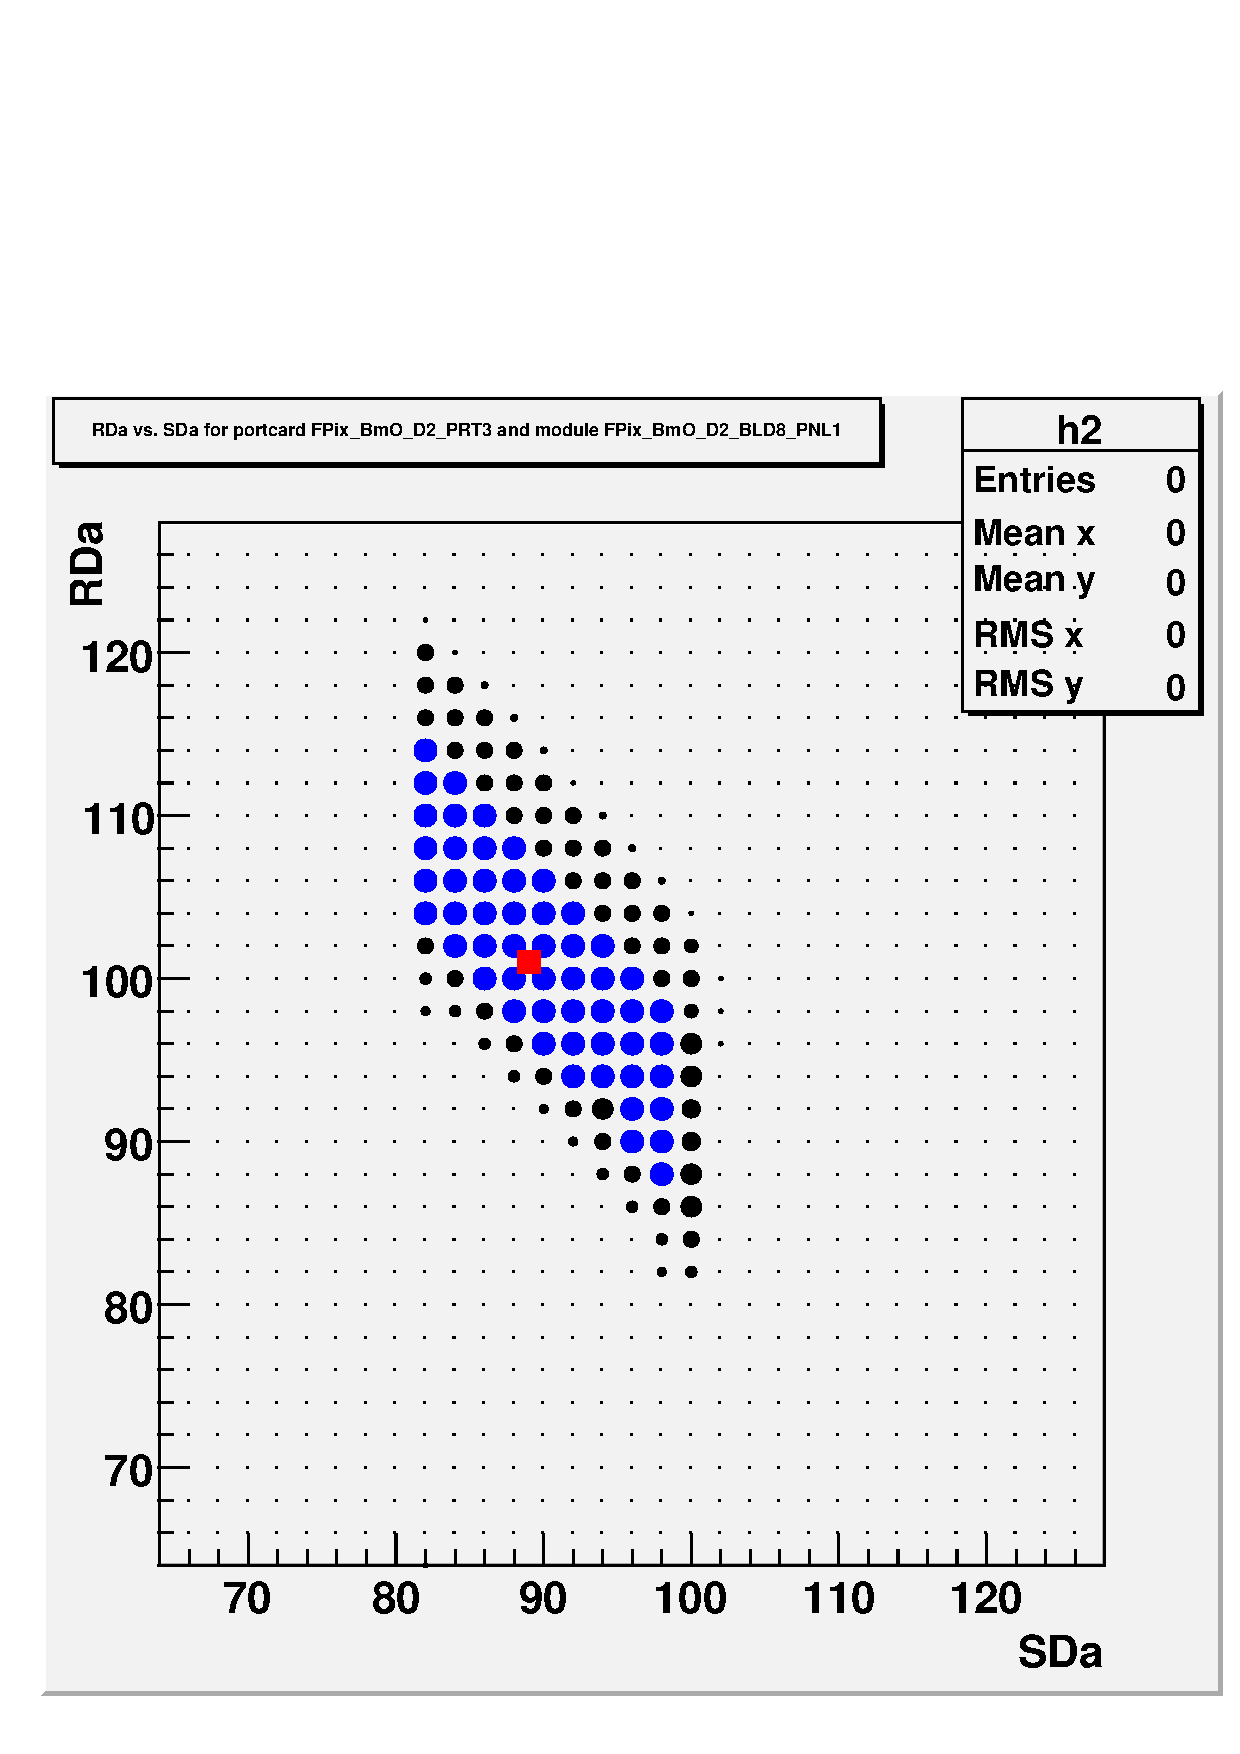
\includegraphics[width=0.8\textwidth]{graph_FPix_BmO_D2_PRT3_FPix_BmO_D2_BLD8_PNL1.pdf}
\end{center}
\caption{
This plot shows efficiency as a function of RDa and SDa. The blue dots indicates areas with 100\% transmission efficiency. The black dots indicated partial efficiency, larger dots have higher efficiency. The red square indicates the point chosen by the algorithm. }
\label{fig:Delay25Scan}
\end{figure}

The calibration succeeds if the algorithm finds an efficient point.  If the efficient band is very thin, it might be because the bias settings of the DOH (DOH\_Ch0Bias\_CLK and DOH\_Ch1Bias\_Data), which read back the result of the programming test, are too low.  The plot can also look bad if the fibers are dirty.

\subsubsection{Results}
This calibration updates the portcard configuration.  The only changes made to the port card settings are for the send data and return data delays.

\subsection{FEDBaselineCalibration}
\label{sec:FEDBaselineCalibration}

\subsubsection{Introduction}
This calibration adjusts the input offset and channel offsets of the optical receivers in the FED such that the black level is adjusted to be near a given target value, normally 450, which is near the midpoint of the dynamic range of the ADC. During this calibration the baseline correction in the FED is turned off. Besides determining the input offset and the channel offsets the algorithm determines address levels for the black and ultra-black levels. This calibration must be run frequently, as the FED baseline is highly temperature dependent. At P5 in 2010-2011, we determined that the automatic baseline correction could cope with changes of 1-2 degrees C.  We monitored the size of the automatic baseline correction with the PixelMonitor tool and reran the FEDBaseline calibration whenever the size of the correction surpassed 100 units.

The calibration is also useful as a debugging tool, as it runs fast and outputs a digitized version of the FED buffer.  

\subsubsection{Procedure}
The FEDBaselineCalibration is an iterative procedure.  In each iteration, the FED signal is read out and digitized, and the baseline calculated.  The input offset and channel offsets of the optical receivers are then adjusted to bring the baseline close to 450 ADC units for each channel.  Because multiple channels share some settings, it may take multiple iterations for the algorithm to converge on settings which yield good baselines for all channels at once. The algorithm is allowed 14 iterations to converge to good settings.

\subsubsection{Parameters}
An example \verb|calib.dat| file for the FEDBaselineCalibration is shown below:

\begin{verbatim}
Mode: FEDBaselineWithPixels
SingleROC
Rows:
0 | 1 | 2 | 3 | 4 | 5 |
6 | 7 | 8 | 9 | 10 |
11 | 12 | 13 | 14 | 15 |
16 | 17 | 18 | 19 | 20 |
21 | 22 | 23 | 24 | 25 |
26 | 27 | 28 | 29 | 30 |
31 | 32 | 33 | 34 | 35 |
36 | 37 | 38 | 39 | 40 |
41 | 42 | 43 | 44 | 45 |
46 | 47 | 48 | 49 | 50 |
51 | 52 | 53 | 54 | 55 |
56 | 57 | 58 | 59 | 60 |
61 | 62 | 63 | 64 | 65 |
66 | 67 | 68 | 69 | 70 |
71 | 72 | 73 | 74 | 75 |
76 | 77 | 78 | 79
Cols:
0 | 1 | 2 | 3 | 4 |
5 | 6 | 7 | 8 |
9 | 10 | 11 | 12 |
13 | 14 | 15 | 16 |
17 | 18 | 19 | 20 |
21 | 22 | 23 | 24 |
25 | 26 | 27 | 28 |
29 | 30 | 31 | 32 |
33 | 34 | 35 | 36 |
37 | 38 | 39 | 40 |
41 | 42 | 43 | 44 |
45 | 46 | 47 | 48 |
49 | 50 | 51
VcalHigh:
100 100 5
Repeat:
10
ToCalibrate:
all
\end{verbatim}

\subsubsection{Output}
The calibration produces a ROOT file containing the digitized FED buffer for each channel at each iteration. An example is shown in Fig \ref{fig:FEDbuffer}.  In addition, summary plots of the baselines of all channels in a FED and the average baselines of all FEDs are saved for each iteration. Example summary plots are shown in Fig \ref{fig:FEDBaselineSummary}.

This output is useful for diagnostic purposes. The digitized FED buffer is expected to contain a TBM header, 16-24 ROC header/trailers (depending on the channel), and a TBM trailer.  The ROC ultrablacks and the blacks should be consistent.  A ragged-looking FED buffer, with inconsistent blacks or ultrablacks, may indicate a bad channel.  A flat FED buffer may also occur if there are problems talking to a given channel.

The calibration succeeds if it converges within 14 iterations.  If the detector is in a good state, the calibration will usually converge in 3 or less iterations.  The calibration may fail if the detector is not thermalized.  Since the baseline is highly temperature dependent, changes to the temperature of the detector will cause the calibration to fail. One should wait 20 minutes after powering on the detector before running the FEDBaselineCalibration.  The calibration may also fail due to a bad channel.  A bad channel may be diagnosed by looking at the baseline summary plots and examining any outliers.  

\subsubsection{Results}
This calibration produces new fedcard settings.

\subsection{AOHBias}
\label{sec:AOHBiasCalibration}

\subsubsection{Introduction}
The AOH bias is a setting on the port card which controls the amount of light sent to the FED.  There is one AOH bias setting per FED channel.  As AOH bias increases, more light is sent, and the ADC values on the FED increase.  At low values of AOH bias, both black and ultrablack do not change with AOH bias, and there is no separation between black and ultrablack levels. At some threshold, the black level begins to increase approximately linearly.  At a higher threshold, the ultrablack level also starts to increase linearly with approximately the same slope.  This behavior is illustrated in Fig.~\ref{fig:AOHBiasScan}.

\begin{figure}
\begin{center}
 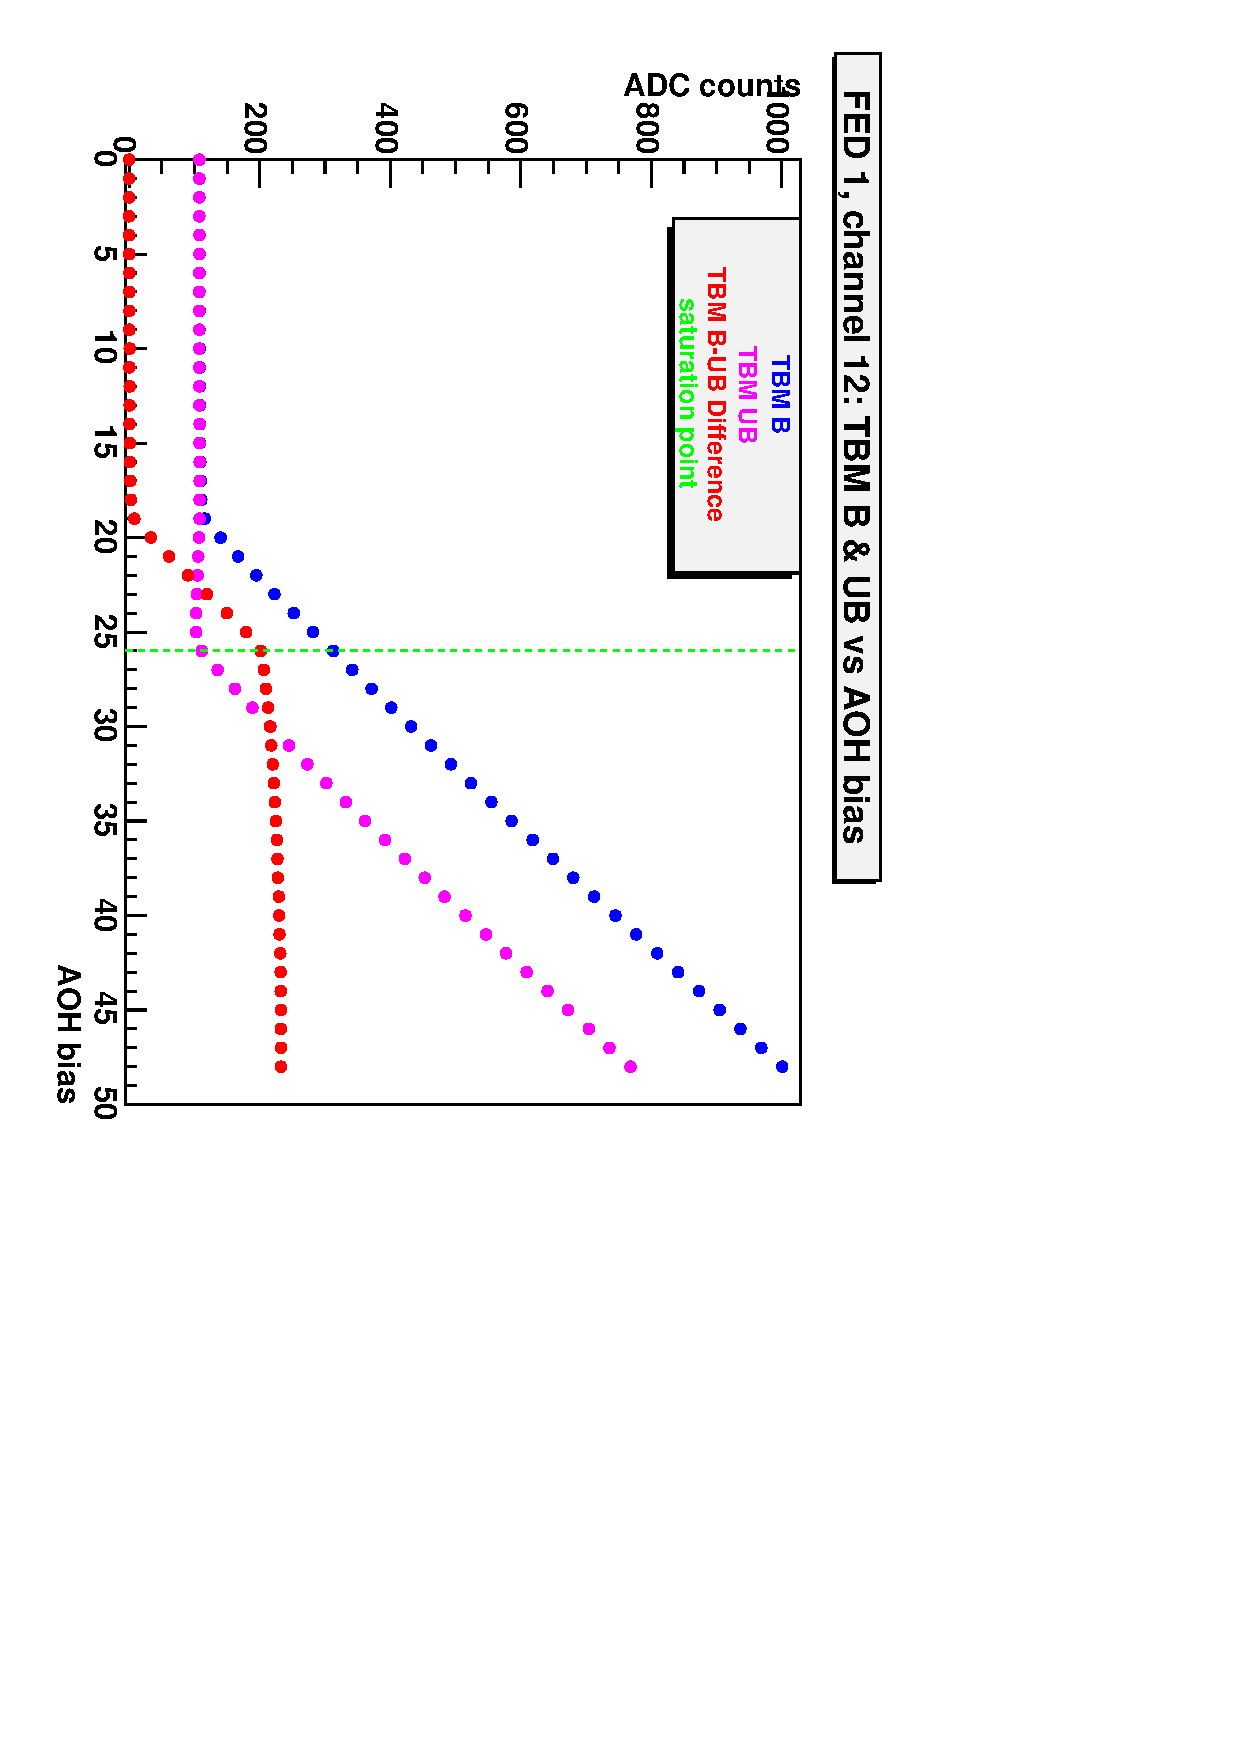
\includegraphics[angle=90,width=0.99\textwidth]{AOHBiasScan.pdf}
\end{center}
\caption{Black and ultrablack levels as a function of AOH bias.}
\label{fig:AOHBiasScan}
\end{figure}

Note that the maximum black-ultrablack separation depends on how the TBM DACs are set.  At low DAC settings, the TBM outputs a signal with relatively low separation; as these settings increase, the separation also increases.  In the AOH bias scan, the black level is independent of the TBM settings.  However, the linear rise of the ultrablack level begins at a later point for higher TBM settings, and hence the black-ultrablack difference saturates at a higher AOH bias value when the TBM DAC settings are higher.

The goal of the AOH bias calibration is to determine an AOH bias setting for each channel that is just high enough to saturate the black-ultrablack difference.  The calibration measures this difference, using black and ultrablack levels from the TBM header and trailer, as a function of AOH bias.  It is important, though, that during the scan the TBM DACs are set at least as high as they will be set in later calibrations and physics runs.  Otherwise, the AOH bias value determined from the saturation point will be too low. TBM settings above those used in this scan will not increase the B-UB separation because the AOH cannot provide more separation.

Temperature variations alter the response of the AOH, essentially shifting the curves in Figure \ref{fig:AOHBiasScan} to the left or right.  In order to provide a margin of error for temperature changes, the AOH bias should be set higher than the saturation value.  A temperature increase of 5 degrees Celcius will shift the curves by about 4 AOH bias counts.  Therefore, by default the chosen AOH bias setting will be 4 counts higher than the saturation value.  This offset is a configurable parameter.

It is also important that the AOH bias not be too high; otherwise the FED offsets could not bring the signal into the dynamic range of the FED. The last part of the AOH bias calibration is to do a coarse baseline adjustment.  The FED channel offsets are set to the center of the range (127), and then the FED optical receiver offsets and AOH bias settings are adjusted to bring all FED baselines into a wide target range.  AOH bias is not decreased below the saturation value unless it is absolutely necessary. The end result is a configuration of AOH bias and FED offset values that puts all FED baselines near the center of the dynamic range, with AOH bias values that allow for a large B-UB separation.  After the AOH bias calibration, the FED baseline calibration should be run to perform fine adjustments of the baseline (using the freedom to move each channel offset).

\subsubsection{Procedure}
This calibration involves many distinct steps.  They are listed in order below.  Each step is performed on each channel being calibrated.
\begin{enumerate}
\item Set the FED channels to the 2V peak-to-peak range in order to provide maximum dynamic range for the AOH bias scan.
\item Turn off the FED automatic baseline correction.
\item Issue \verb|ClrCal| to all ROCs, and disable hits with the control register on all ROCs, to ensure that no hits are output.
\item Set all TBM DACs to high values.  These values may be specified as parameters in \verb|calib.dat|.
\item Set all FED optical receiver input offsets to the highest useful value (the setting that minimizes the FED ADC values, without impairing the B-UB separation).  This value is configurable, and it defaults to 8 (on a scale from 0 to 15).  Also, all channel offsets are set their maximum value, 255. \label{item:FEDReceiverOffset}
\item Issue \verb|LRES| and \verb|CLRES| commands to all FEDs to clear the transparent data.  This ensures that no stale data is sitting in the buffer.
\item Loop over AOH bias values.  Attempt to decode the transparent buffer on each trigger, assuming the correct number of ROCs and no hits. That is, find the TBM header, and verify that the TBM trailer is in the right place.  When decoding is successful, record the start slot of the TBM header and trailer.  On each channel, this slot should be the same for all triggers.  The reason for this step is to find the time slots for later use in reading out TBM B and UB levels, even at low AOH bias settings where full decoding would fail. If no reliable time slots are found\footnote{A time slot is considered found if the most common start slot occurs on at least 95\% of the triggers.  Alternatively, if the two most frequent time slots differ by 1 (due to a jumping clock) and together account for at least 95\% of triggers, then the time slots are considered found, and TBM B and UB are sampled only in those time slots which are known to be B or UB for either of the two start slots.} on a channel, this channel is considered failed, and it is ignored in the rest of the routine.
\item Now scan over AOH bias again, this time to record the TBM B and UB levels at each setting, using the time slots recorded in the previous step.\footnote{If good time slots were not found on a given channel, only the black level will be recorded and plotted.  It is taken from the first 10 slots of the transparent buffer, rather than from the TBM header and trailer.  This plot is for diagnostic purposes only; it is not used in generating new configuration settings.} During the scan, if the signal goes out of range high or low, the FED channel offset is adjusted to bring it back into range, if possible.  Since only the B-UB difference is of interest, coherent shifts in B and UB do not matter.  The FED optical receiver offset is not adjusted during the scan -- it remains at the high setting described in step \ref{item:FEDReceiverOffset}.
\item Output plots of the TBM black and ultrablack, and the difference, as a function of AOH bias, to a ROOT file.  Figure~\ref{fig:AOHBiasScan} is an example of the plots produced.  Find the AOH bias value at which the B-UB difference saturates (defined as a reduction in the slope to less than 20\% of its maximum value).  Set each AOH to its saturation value plus the offset defined by the parameter \verb|SaturationPointOffset| (which defaults to 4).
\item Set FED channels back to the 1V peak-to-peak range, for those channels which were originally set at 1V in the FED configuration file.  This is done so that the coarse baseline adjustment will be done with the range that will be used for future data-taking.
\item Set FED optical receiver input offsets to 0 (lowest value, corresponding to highest FED ADC values), and all channel offsets to 127 (middle of the range).  The channel offset will be left at 127 for the rest of the routine.
\item Measure black levels on all channels.  On each FED optical receiver, if any channel has a black level above the target range, increase that receiver's offset by one.  If not, do nothing.  Repeat this until all channels have black levels in or below the target range, or have a receiver offset equal to the maximum value described in step \ref{item:FEDReceiverOffset} (defaults to 8).  The idea here is to ensure that no AOH bias value will have to be decreased to place the black level in the target range (unless this is absolutely necessary because the receiver offset cannot be increased further).
\item Again measure the black levels on all channels.  If a channel's black level is within the target range, that channel is done.  If it is above or below the target range, decrease or increase AOH bias.  Repeat this until all channels are within range.  (Or, if two adjacent AOH bias values produce black levels that straddle the target range, chose the one that is closer to the target.)  AOH bias should not have to decrease unless the FED receiver input offset was at maximum.  If it does decrease, a warning is generated in
the summary at the end of the calibration. 
\item Turn FED automatic baseline correction back on.
\item Write new config files for all port cards and FEDs with at least one successfully calibrated channel.
\item Print a summary to the screen.  Thus summary gives the number of successful and failed channels, statistics on the new settings for successful channels, descriptions of the errors on unsuccessful channels, and warnings for channels on which the final AOH bias setting is below the saturation point.
\end{enumerate}

\subsubsection{Parameters}
A number of parameters in \verb|calib.dat| may be used to control the calibration.

Only two ``standard" parameters are used.  The ``\verb|Repeat:|" parameter determines the number of triggers in each step (at each AOH bias scan point and when measuring black levels in the coarse baseline adjustment).  The channel list is used to determine which channels are calibrated.  Note that the rows, columns, and DAC scan settings in \verb|calib.dat| are completely ignored.

Many other optional parameters may be set.  All have default values which will be used if the parameter is not set.  These parameters, their defaults, and their functionality are given in Table~\ref{tab:AOHBiasParameters}.

\begin{table}
\centering
\caption{Optional parameters for AOH bias calibration.}
\label{tab:AOHBiasParameters}
\begin{tabular}{l@{~~~~}r@{~~~~}l}
\hline
\hline
Parameter & Default & Description \\
\hline
ScanMin                     &   0 & Low end of AOH bias scan range \\
ScanMax                     &  50 & High end of AOH bias scan range \\
ScanStepSize                &   1 & Step size for AOH bias scan \\
TargetBMin                  & 412 & Allowed range for the coarse baseline \\
TargetBMax                  & 612 & adjustment at the end of this calibration \\
SaturationPointOffset       &   4 & After finding the saturation point, this \\
                            &     & number is added to get the AOH bias setting \\
                            &     & (but before adjusting the black level). \\
MaxFEDReceiverInputOffset   &   8 & Largest allowed value of the FED receiver \\
                            &     & input offset, which can range from 0 to 15 \\
SetAnalogInputBias          & 200 & TBM settings to use \\
SetAnalogOutputBias         & 120 & for all channels -- \\
SetAnalogOutputGain         & 200 & all 3 should be set high \\
printFEDRawData             &  no & Whether to print decoded transparent buffer \\
printFEDOffsetAdjustments   &  no & Whether to print when the FED offsets change \\
printAOHBiasAdjustments     &  no & Whether to print a message when the AOHBias \\
                            &     & is changed during the baseline adjustment \\
\hline
\hline
\end{tabular}
\end{table}

\subsubsection{Output}
\subsubsection{Results}

\subsection{AOHGain}

\subsubsection{Introduction}

The AOH gain is a setting for each optical link (from detector to FED) that has just 4 possible settings (0, 1, 2, 3).  This setting does not change the black level.  Instead, it scales the size of deviations from the black level, expanding or shrinking the signal.  Larger settings correspond to larger deviations.  In particular, the separation between black and ultrablack levels will be larger at a larger gain.  Settings on the TBMs and ROCs will be the primary means of adjusting the ultrablack to the desired level, but the AOH gain must be set large enough in order to make possible a low enough ultrablack.  However, AOH gain should not be set too high since larger settings will increase the power drawn, and larger settings are intended to be used to compensate for radiation damage over time.

The aim of this calibration is to set the AOH gain at the lowest level that will allow the TBM UB level to be low enough.  The three TBM DACs (described in Sec.~\ref{sec:TBMUB}) are set to high values.  Then, for each FED channel, TBM UB is recorded as a function of AOH gain.  To choose an AOH gain setting, the calibration selects the smallest value that produces an UB below a user-defined threshold.

\subsubsection{Procedure}

The calibration consists of the following steps:
\begin{enumerate}
\item Issue \verb|ClrCal| to all ROCs, and disable hits with the control register on all ROCs, to ensure that no hits are output.
\item Issue \verb|LRES| and \verb|CLRES| commands to all FEDs to clear the transparent data.  This ensures that no stale data is sitting in the buffer.
\item Set all TBMs to high values.  The user may specify these values; otherwise defaults will be used.
\item Scan over values of AOH gain.  Attempt to decode the transparent buffer on each trigger, assuming the correct number of ROCs and no hits. That is, find the TBM header, and verify that the TBM trailer is in the right place.  If decoding is successful, record the UB values in the TBM header and trailer (5 values per trigger, 3 from the header and 2 from the trailer).  If decoding is unsuccessful, ignore that trigger, and don't record anything.  For each channel, a plot of this scan is output to a ROOT file.
\item Analyze the recorded scan data on each FED channel, looking for the smallest AOH gain where the UB is below the threshold specified by the user.  This is the recommended AOH gain value.  (If all values were above the threshold, set the AOH gain to 3 and generate an error.)
\item On dual TBMs, check whether we can reduce the difference in UB levels by raising one of the two AOH gains by 1.  If so, do it.  This minimizes the spread between ultrablack levels on dual TBMs.  (Since the two channels share the same TBM DAC settings, there is no other way to independently adjust the TBM UB levels.)
\item Write out new port card configuration files with the new AOH gain settings.
\item Print out a summary.
\end{enumerate}

\subsubsection{Parameters}
A number of parameters in \verb|calib.dat| may be used to control the calibration.

Only two ``standard" parameters are used.  The ``\verb|Repeat:|" parameter determines the number of triggers in each step of the scan.  The channel list is used to determine which channels are calibrated.  Note that the rows, columns, and DAC scan settings in \verb|calib.dat| are completely ignored.

Many other optional parameters may be set.  All have default values which will be used if the parameter is not set.  These parameters, their defaults, and their functionality are given in Table~\ref{tab:AOHGainParameters}.

\begin{table}
\centering
\caption{Optional parameters for AOH gain calibration.}
\label{tab:AOHGainParameters}
\begin{tabular}{l@{~~~~}l@{~~~~}l}
\hline
\hline
Parameter & Default & Description \\
\hline
SetAnalogInputBias   & 160                & Value of AnalogInputBias to set on all channels. \\
SetAnalogOutputBias  & 110                & Value of AnalogOutputBias to set on all channels. \\
SetAnalogOutputGain  & 240                & Value of AnalogOutputGain to set on all channels. \\
MaxTBMUB             & 100                & TBM UB threshold.  AOH gain will be set so \\
                     &                    & that TBM UB is below this level. \\
printFEDRawData      & no                 & Whether to print decoded transparent buffer \\
printScan            & no                 & Whether to print TBM UB levels \\
                     &                    & for each AOH gain \\
\hline
\hline
\end{tabular}
\end{table}

\subsubsection{Output}
\subsubsection{Results}

\subsection{TBMUB}
\label{sec:TBMUB}

\subsubsection{Introduction}

With the black level set at 512 by the baseline calibration and automatic baseline correction, the next step is to set the ultrablack levels appropriately.  We first adjust DACs on the TBM to set the TBM header and trailer ultrablack to an appropriate value. (Experience from forward testing suggests that a value of 120 to 150 is good.)

There are three DAC settings on the TBM, all of which affect the ultrablack level.  Higher values of these DACs correspond to lower ultrablack (and greater B-UB separation).  Figure~\ref{fig:tbm-anal-dacs} shows how these DACs affect the output of the TBM.  The \verb|AnalogOutputGain| setting alters the levels of the TBM header and trailer, but not the signals from the ROCs.  The \verb|AnalogInputBias| setting affects both ROC and TBM signals, but it changes ROC signals more than TBM signals.  The \verb|AnalogOutputBias| setting affects ROC and TBM signals equally. The TBM UB level may be adjusted by any or all of these three DAC settings.

\begin{figure}
\begin{center}
 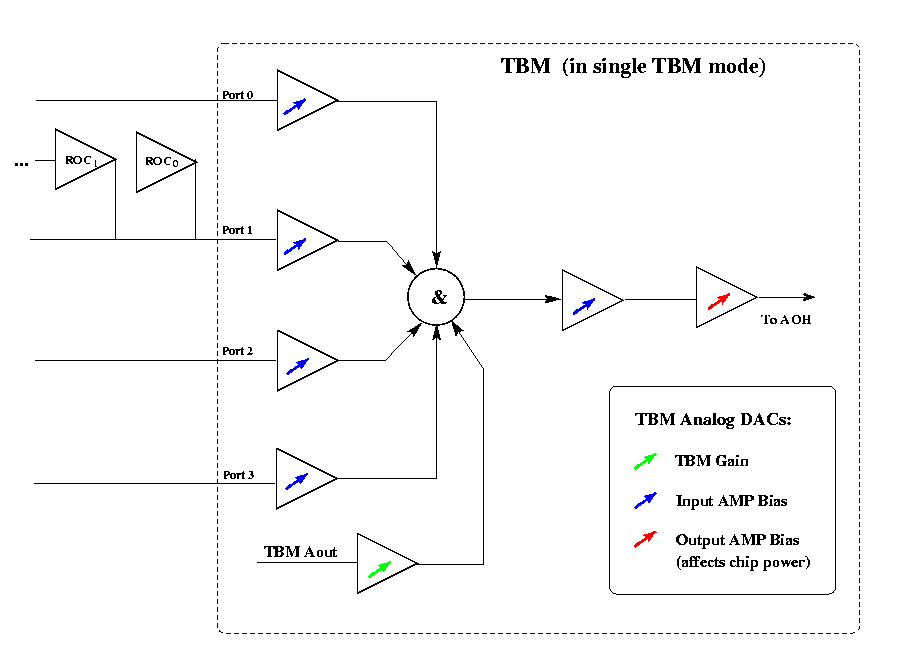
\includegraphics[width=0.99\textwidth]{tbm-anal-dacs.png}
\end{center}
\caption{Diagram illustrating how the TBM DACs affect the output of the TBM.
AnalogInputBias is referred to as Input AMP Bias (blue arrows),
AnalogOutputBias is referred to as Output AMP Bias (red arrows),
and AnalogOutputGain is referred to as TBM Gain (green arrows).}
\label{fig:tbm-anal-dacs}
\end{figure}

Although higher DAC values generally produce lower ultrablack levels, at very high DAC values the ultrablack level may actually increase.  In particular, \verb|AnalogOutputBias| should not exceed $\sim$128.  If the calibration finds multiple settings that give the target ultrablack level, it will choose the lower settings.

The TBM UB calibration routine can run in either of two modes, as selected by the user:
\begin{enumerate}
\item Fix two DAC settings and scan the third.  The user selects which DAC to scan and specifies the scan range.  Optionally, the other two DACs may be given particular settings for all ROCs; otherwise the values stored in the configuration database will be used.
\item Scan all three settings simultaneously.  The user selects a scan range for each DAC, as well as the number of scan points.  During the scan, all three settings are moved simultaneously and proportionally through their ranges.  Specifically, for scan point $i = \{0, 1,..., N-1\}$, the value of DAC $d$ is
\begin{equation}
v_{d}(i) = min_{d} + \frac{i}{N-1} \times (max_{d}-min_{d})
\end{equation}
where $N$ is the number of scan points and $min_{d}$ and $max_{d}$ are the minimum and maximum scan values for DAC $d$.
\end{enumerate}
In either mode, the calibration searches for DAC settings that put the TBM UB at the target level. (This level defaults to 135, and may be changed by the user.)  The second mode, where all three settings are varied simultaneously, is recommended.

Dual TBMs are a special case.  The two channels on a dual TBM share the same DAC settings, so they cannot be adjusted independently.  Therefore the TBM settings cannot be adjusted to simultaneously put both channels' UB at the target level.  For dual TBMs, we set the DACs so that one channel is at the target UB level, and the other is below.

\subsubsection{Procedure}

The calibration consists of the following steps:
\begin{enumerate}
\item Issue \verb|ClrCal| to all ROCs, and disable hits with the control register on all ROCs, to ensure that no hits are output.
\item Issue \verb|LRES| and \verb|CLRES| commands to all FEDs to clear the transparent data.  This ensures that no stale data is sitting in the buffer.
\item Scan over DAC values as specified by the user, either varying just one DAC or varying all three simultaneously.  Attempt to decode the transparent buffer on each trigger, assuming the correct number of ROCs and no hits. That is, find the TBM header, and verify that the TBM trailer is in the right place.  If decoding is successful, record the UB values in the TBM header and trailer (5 values per trigger, 3 from the header and 2 from the trailer).  If decoding is unsuccessful, ignore that trigger, and don't record anything.  For each FED channel, a plot of this scan is output to a ROOT file.
\item Analyze the recorded scan data on each FED channel, looking for the point where the measured UB crosses the target level.  When the crossing is found, interpolate between the nearest scan points for the best DAC settings. If no crossing is detected, the channel is considered failed.  If multiple crossings are detected, a warning is generated for that channel.  New DAC settings will still be generated if the scan contains some data -- either the value that puts the UB closest to the target, or the leftmost crossing point (lowest DAC values) if there are more than one.
\item On single TBMs, the new DAC values are the values at this crossing point. On dual TBMs, the new DAC values are the higher of the two sets of values found on the two FED channels for that TBM; this ensures that both UB levels will be at or below the target.  If only one of the two channels was on the list of channels to calibrate, then the new DAC value is based on the one channel, and a warning is generated.  A warning is also generated if both channels were successful, but the DAC values were too far apart.
\item Write out new TBM configuration files for the modules with new DAC settings (including any settings which were not varied during the scan).
\item Print out a summary.
\end{enumerate}

\subsubsection{Parameters}
A number of parameters in \verb|calib.dat| may be used to control the calibration.

Only two ``standard" parameters are used.  The ``\verb|Repeat:|" parameter determines the number of triggers in each step of the scan.  The channel list is used to determine which channels are calibrated.  Note that the rows, columns, and DAC scan settings in \verb|calib.dat| are completely ignored.

One other parameter is required.  The parameter \verb|DACToScan| must be set to \verb|AnalogInputBias|, \verb|AnalogOutputBias|, \verb|AnalogOutputGain|, or \verb|All|.  Selecting \verb|All| will scan all three DACs simultaneously; otherwise just one is scanned.

Many other optional parameters may be set.  All have default values which will be used if the parameter is not set.  These parameters, their defaults, and their functionality are given in Table~\ref{tab:TBMUBParameters}.

\begin{table}
\centering
\caption{Parameters for TBM UB calibration.  All except DACToScan are optional.}
\label{tab:TBMUBParameters}
\begin{tabular}{l@{~~~~}l@{~~~~}l}
\hline
\hline
Parameter & Default & Description \\
\hline
DACToScan            & N/A                & Which of the three TBM DACs to scan, or ``All" \\
\hline
\multicolumn{3}{c}{DACToScan $\neq$ All} \\
ScanMin              & 0                  & Low end of DAC scan range \\
ScanMax              & 255                & High end of DAC scan range \\
ScanStepSize         & 5                  & Step size for DAC scan \\
SetAnalogInputBias   & [empty]            & If not set, leave AnalogInputBias unchanged. \\
                     &                    & Otherwise, set it to the specified value and\\
                     &                    & change in the output configuration file. \\
SetAnalogOutputBias  & [empty]            & If not set, leave AnalogOutputBias unchanged. \\
                     &                    & Otherwise, set it to the specified value and\\
                     &                    & change in the output configuration file. \\
SetAnalogOutputGain  & [empty]            & If not set, leave AnalogOutputGain unchanged. \\
                     &                    & Otherwise, set it to the specified value and\\
                     &                    & change in the output configuration file. \\
\hline
\multicolumn{3}{c}{DACToScan = All} \\
MinAnalogInputBias   & 0                  & Minimum AnalogInputBias value during scan \\
MaxAnalogInputBias   & 255                & Maximum AnalogInputBias value during scan \\
MinAnalogOutputBias  & 0                  & Minimum AnalogOutputBias value during scan \\
MaxAnalogOutputBias  & 128                & Maximum AnalogOutputBias value during scan \\
MinAnalogOutputGain  & 0                  & Minimum AnalogOutputGain value during scan \\
MaxAnalogOutputGain  & 255                & Maximum AnalogOutputGain value during scan \\
\hline
\multicolumn{3}{c}{Any DACToScan Setting} \\
ScanNumSteps         & 52                 & Number of scan steps -- will override \\
                     &                    & ScanStepSize setting, if present \\
TargetUB             & 135                & Desired TBM UB level \\
DualTBMMaxScanStepDiff& 6                 & If the difference in scan steps between the final DAC\\
                     &                    & settings on the two channels of a dual TBM\\
                     &                    & exceeds this value, a warning is generated. \\
printFEDRawData      & no                 & Whether to print decoded transparent buffer \\
printScan            & no                 & Whether to print TBM UB levels \\
                     &                    & for each DAC setting \\
\hline
\hline
\end{tabular}
\end{table}

\subsection{ROCUB}

\subsubsection{Introduction}

This calibration sets the ultrablack level for each ROC equal to the corresponding TBM's ultrablack level.

There are two DAC settings on the ROC which affect the ultrablack level. Higher values of these DACs correspond to lower ultrablack (and greater B-UB separation).  \verb|VIbias_roc| affects UB, address levels, and pulse height.  \verb|VIbias_DAC| affects UB and address levels, but not pulse height.  In this routine, \verb|VIbias_DAC| is scanned while \verb|VIbias_roc| is fixed.

\subsubsection{Procedure}

This calibration is very similar to the TBM UB calibration, except that each individual ROC is analyzed.  It consists of the following steps:

\begin{enumerate}
\item Issue \verb|LRES| and \verb|CLRES| commands to all FEDs to clear the transparent data.  This ensures that no stale data is sitting in the buffer.
\item Scan over values of \verb|VIbias_DAC|.  (If the calib.dat file specified a fixed value of \verb|VIbias_roc|, this is also set.)  Each time after \verb|VIbias_DAC| is changed, issue \verb|ClrCal| to all ROCs, and disable hits with the control register on all ROCs, to ensure that no hits are output (so any hits specified in the configuration file are ignored).  Attempt to decode the transparent buffer on each trigger, assuming the correct number of ROCs and no hits.  That is, find the TBM header, and verify that the TBM trailer is in the right place.  If decoding is successful, record the UB values in the TBM header and trailer, and for each ROC.  If decoding is unsuccessful, ignore that trigger, and don't record anything.  For each ROC, a plot of this scan is written to a ROOT file.
\item Analyze the recorded scan data on each ROC, looking for the point where the measured ROC UB equals the UB level on the corresponding TBM. When the ROC UB crosses the TBM UB, interpolate between the nearest scan points for the best \verb|VIbias_DAC| setting. If no crossing is detected, the ROC is considered failed.  If multiple crossings are detected, a warning is generated for that ROC.  A new \verb|VIbias_DAC| setting will still be generated if the scan contains some data -- either the value that puts the ROC UB closest to the TBM UB, or the leftmost crossing point (lowest \verb|VIbias_DAC| value) if there are more than one.
\item Write out new ROC configuration files with the new \verb|VIbias_DAC| settings.  If \verb|VIbias_roc| was modified by the user, the output files will contain this new value, too.
\item Print out a summary.
\end{enumerate}

\subsubsection{Parameters}
A number of parameters in \verb|calib.dat| may be used to control the calibration.

The various ``standard" parameters are used in this calibration.  The ``\verb|Repeat:|" parameter determines the number of triggers in each step of the scan.  The ROC list is used to determine which ROCs are calibrated.

A line like
\begin{verbatim}
Scan: VIbias_DAC 80 200 5
\end{verbatim}
must be included to specify the scan range (first two numbers) and step
size (last number).

Optionally, \verb|VIbias_roc| may be set with a line like
\begin{verbatim}
Set: VIbias_roc 150
\end{verbatim}

Any hits specified in \verb|Rows:| and \verb|Columns:| will be ignored.  (This is done by explicitly clearing them.)  The \verb|Rows:| and \verb|Columns:| parameters should be empty; otherwise the calibration will work but will print a warning message.

Some optional parameters may also be set.  All have default values which will be used if the parameter is not set.  These parameters, their defaults, and their functionality are given in Table~\ref{tab:ROCUBParameters}.

\begin{table}
\centering
\caption{Optional parameters for ROC UB equalization calibration.}
\label{tab:ROCUBParameters}
\begin{tabular}{l@{~~~~}l@{~~~~}l}
\hline
\hline
Parameter & Default & Description \\
\hline
printFEDRawData      & no                 & Whether to print decoded transparent buffer \\
printScan            & no                 & Whether to print TBM UB levels \\
                     &                    & for each DAC setting \\
\hline
\hline
\end{tabular}
\end{table}

\subsubsection{Output}
\subsubsection{Resultss}

\subsection{AddressLevelCalibration}

\subsubsection{Introduction}
The address level determination determines the values used by the FED to encode the transparent data. This include address levels for the pixel addresses, TBM header and trailer levels, and the black and ultrablack levels.

Pixels are scanned to make sure that we probe combinations  of address levels that could potentially cause problems, such as transitions from high to low levels and vice versa.

Due to limitations in the size of the FIFO1 transparent  data size of 512 clocks, we can not even take one hit per ROC unless the timing is adjusted such that the  start of the pulse train comes relatively early, i.e. in the first 20 or so clock cycles. Recall, each ROC, with one hit takes 9 clock cycles to read out. Then with 24 ROCs in a module we need 216 clock cycles just to read out the  hits. Plus about 16 clock cycles to read out the TBM headers

\subsubsection{Procedure}
\subsubsection{Parameters}
\subsubsection{Output}
\subsubsection{Results}

%\subsubsection{Data volume and time estimate}

%The worst case scenario for an address level calibration is one BPIX crate. We have 16 FED cards in one crate, and we can assume that all of them are fully populated. This means that we have $16\times 36=576$ links. As we read out this data in transparent mode we will read 1024 words per event (even though the transparent data is only 512 bytes long). This means a total of  235926 bytes. If we want to go thought all pixel we have to read out 4160 times this data volume for a total of 9,4 GB. At a speed of 10 MB/s this will take 940 s. 

%Assuming that we change the transparent data FIFO to be 1024 bytes. Then we can easily fit 4 hits into each ROC. This then cuts the readout time by a factor of 4 as we will need exactly 1/4 the number of triggers. This then becomes 235 seconds. 

%We can also use different patters that used fewer pixel hits. But one has to take care to have all relevant transitions.


\subsection{PixelAlive}
\label{sec:PixelAliveCalib}
\subsubsection{Introduction}
The pixel alive calibration loops over pixel, inject charge, for a fixed VCal setting. The data is analyzed to produce an efficiency map that displays the efficiency for each pixel on a plaquette.

\subsubsection{Procedure}
\subsubsection{Parameters}
\subsubsection{Output}
\subsubsection{Results}

To analyze the data, go to PixelAnalysisTools/test and do
\begin{verbatim}
./bin/linux/x86/PixelAnalysis.exe PixelAliveAnalysis.xml <runnum>
\end{verbatim}
You can also specify the exact configuration file you would like to use, e.g. configuration/PixelAliveAnalysis\_FPix.xml.

You can scan over multiple WBCs when taking this data and analyze the data from all the WBCs summed together or only one of them using the ChooseWBC option in the configuration xml file. To measure absolute thresholds, use the in-time WBC and the following one.  To measure the in-time threshold, use the in-time WBC only.

\subsection{SCurve}
\label{sec:SCurveCalibration}

\subsubsection{Introduction}
The SCurve calibration is similar to the PixelAlive, where we in addition loop over the VCal setting for each pixel. The data is analyzed to produce an efficiency as a function of the VCal setting.

To analyze the data, go to PixelAnalysisTools/test and do

\begin{verbatim}
./bin/linux/x86/PixelAnalysis.exe SCurve <runnum>
\end{verbatim}

\subsubsection{Procedure}
\subsubsection{Parameters}
\subsubsection{Output}
\subsubsection{Results}

You can scan over multiple WBCs when taking this data and analyze the data from all the WBCs summed together or only one of them using the ChooseWBC option in the configuration xml file. To measure absolute thresholds, use the in-time WBC and the following one.  To measure the in-time threshold, use the in-time WBC only.

\subsection{GainCalibration}
\label{sec:GainCalibration}

\subsubsection{Introduction}
The Gain calibration is similar to the SCurve calibration, where instead of measuring the efficiency as a function of VCal we look at the charge (ADC value) as function of the VCal.

\subsubsection{Procedure}
\subsubsection{Parameters}
\subsubsection{Output}
\subsubsection{Results}

To analyze the data, go to PixelAnalysisTools/test and do one of the following: 
\begin{verbatim}
./bin/linux/x86/PixelAnalysis.exe Gain <runnum>
\end{verbatim}

You can scan over multiple WBCs when taking this data and analyze the data from all the WBCs summed together or only one of them using the ChooseWBC option in the configuration xml file. To measure absolute thresholds, use the in-time WBC and the following one.  To measure the in-time threshold, use the in-time WBC only.

%\subsubsection{Practical issues}

%If you get a lot of ``Time Out Error'' messages it could be because you don't have the right channels enabled on the FED. Or more specifically that you have enables channels that are not connected.

%\subsection{Iana vs. Vana Calibration}

%A calibration called ``Iana'' is implemented to  scan Vana and measure the analog current, Iana. As the power distribution for the low voltage is  done per portcard for the forward pixels ({\it need to add how this works for BPix.}) this calibration works in parallel on a ROC at the time on each of the portcards. The current changes we are  measuring is of the order 50 mA as you go from Vana=0 to Vana=255. The A4603 power modules has a resolution of about 7 mA. We perform this  measurement when all other ROCs are configured to their default values. Hence, we measure the current changes on top of a current of several amperes. (I performed trials were I lowered Vana on all other ROCs to reduce the current, but it does not really improve the measurements.) Hence, we have to take the data and fit it in order to  interpolate between the points. (It takes a  long time to do these measurments as one has to wait up to 6 seconds before the current measurement is stable. This should also be brought up with CAEN.)

%\begin{figure}
%\begin{center}
%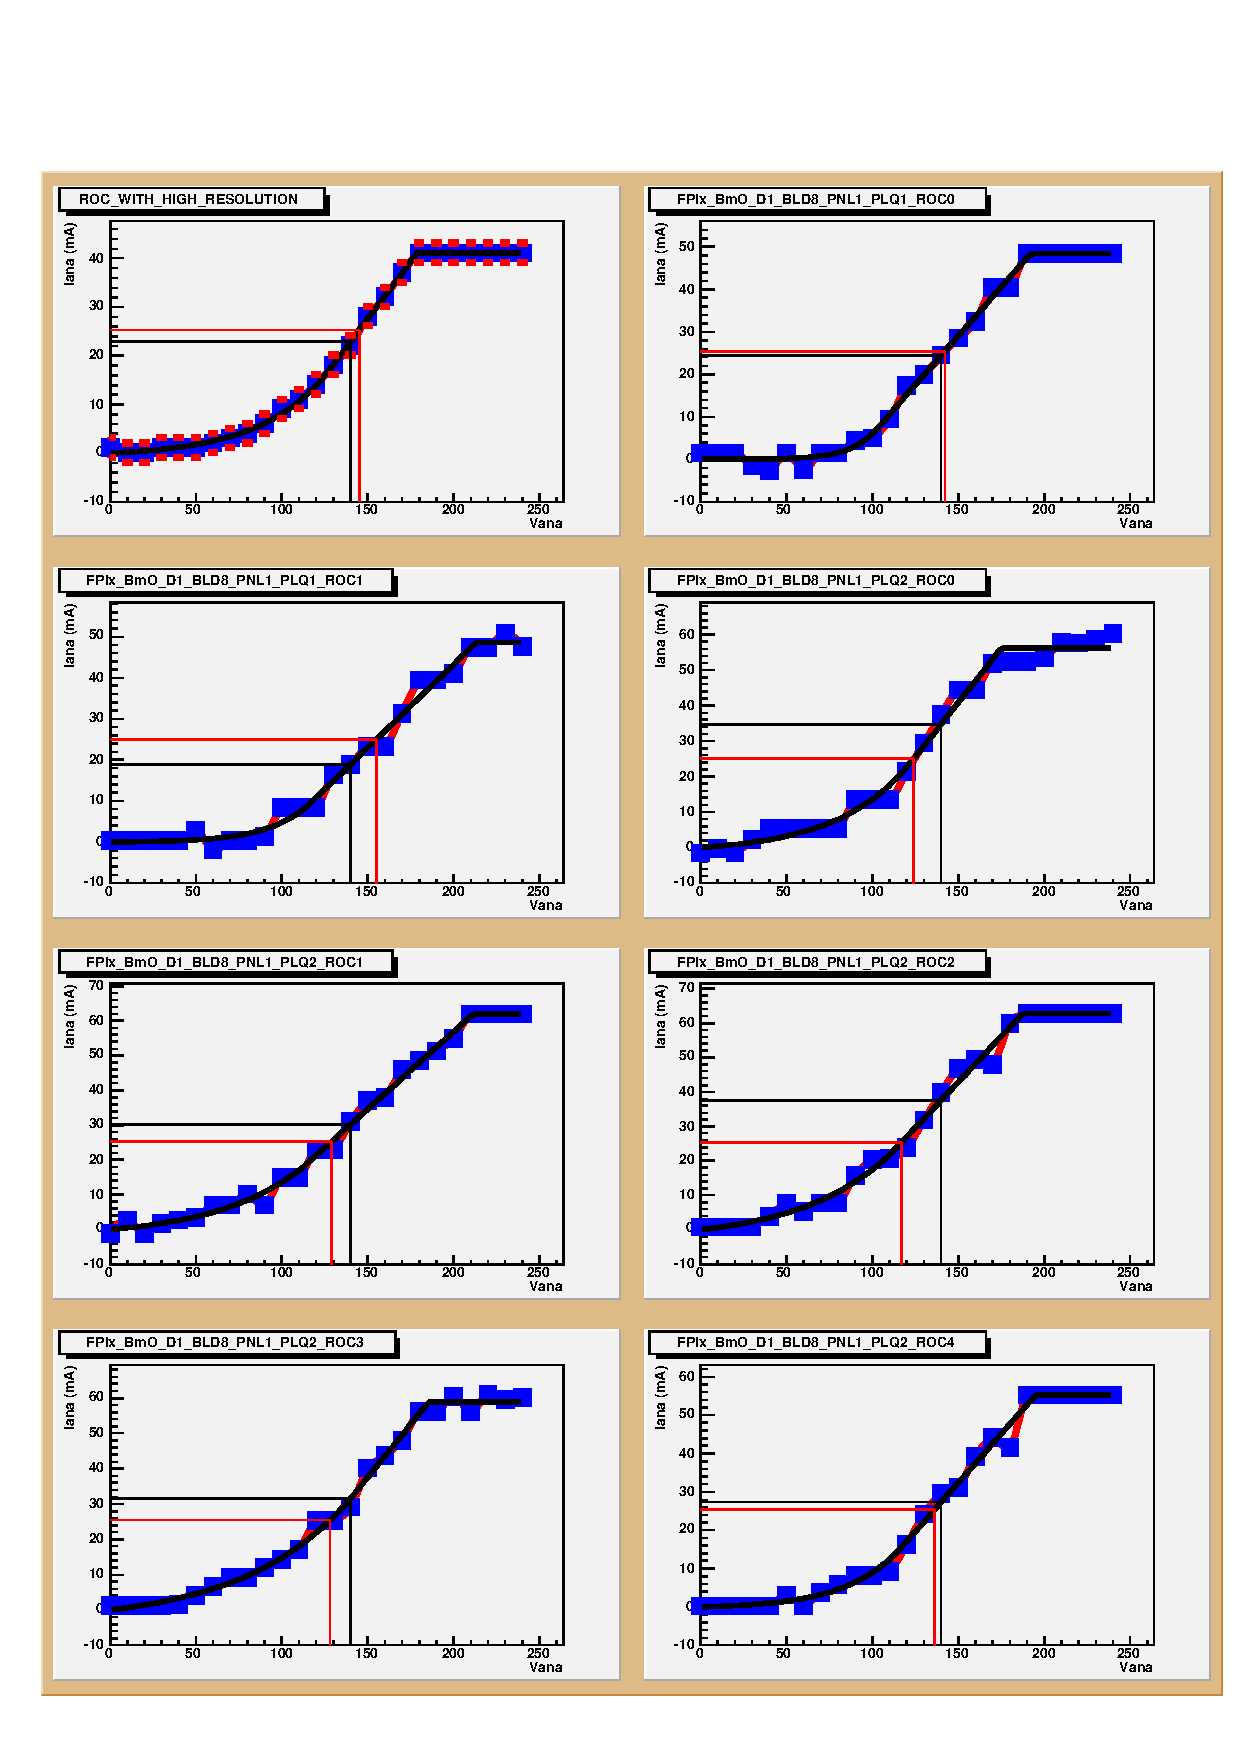
\includegraphics[width=0.85\linewidth]{IanavsVana}
%\end{center}
%\caption{This figure shows the measured analog current, Iana, vs the Vana setting for a few ROCs. The top left plot shows  the Iana measured for one ROC with the A1715 power supply that has a better resolution. The black lines indicate the default setting (Vana=140) used in the configuration when this data was taken.  The red line indicate the setting that gives a analog current of 25 mA.}
%\label{fig:IanavsVana}
%\end{figure}


%To analyze the data we fit it to a functional form. After some experimentation I came up with the following. I divide the range of Vana values into 3 ranges, compare Fig.~\ref{fig:IanavsVana}. In the high range Iana is taken to be a constant. In the low range Iana is taken to be a constant plus an exponential.  In the middle range Iana depends linearly on Vana, and the function is required to be continuous. In addition the function is required to have a continuous derivative as it goes between the low and middle region. This function has 5 free parameters that are determined  in the fit.

%First the raw data is fit to this form. After doing this fit the offset at Vana=0 is subtracted and the data is refit and plotted. These are the fits shown in Fig.~\ref{fig:IanavsVana}.

%A black line is used to indicate where the current used for the default Vana setting (Vana=140). In red is shown where you should set Vana to get an analog current of 25 mA.


\subsection{VcThrCalDel}%
\label{sect:VcThrCalDelCalibration}

\subsubsection{Introduction}
These settings are ROC wide and a few pixels are selected and a scan over the CalDelay and VcThreshold setting is performed. For each setting, triggers are taken and data is looked at using FIFO3 to see how many hits we had on each ROC.  In order for this algorithm to work the address levels for  black and ultra-black has to be set. (There is also an implementation that uses the FIFO1, it does not need address levels.)

We point out that CalDel is {\it only} relevant for calibration data taken with charge injection. The CalDel setting controlls the time in which the charge is injected into the pixels. For real data we will have to adjust the timing, e.g. using the delay 25 settings from the trigger. However, for data taken with charge injection this delay is important.

This calibration performs a 2-D scan of CalDel vs VcThr. For large VcThr, which corresponds to low thresholds, we get lots of noise and the ROC digital readout basically shuts down and we don't see any hits. For lower values of VcThr we get in the range of CalDel values that corresponds to the WBC used. For larger thresholds this curve 'bends' to lower values of CalDel. As this curresponds to a higher threshold the signal reaches the threshold later and hence we need to use a smaller  CalDel, i.e. inject the signal earlier.

\subsubsection{Procedure}
\subsubsection{Parameters}
An example configuration file is shown below.
\begin{verbatim}

Mode: ThresholdCalDelay
Rows:
10 | 20 
Cols:
10 | 20
VcalHigh
Scan: VcThr 0 255 8
Scan: CalDel 0 255 8
Set: Vcal 50
Repeat: 10
ToCalibrate:
all
\end{verbatim}

\subsubsection{Output}

In addition to the DAC settings the calibration produces the output file {\tt VcThrCalDelaySummary.txt} which lists all the ROCs that were used in the calibrations. For each of the ROCs there is a corresponding file, named like  {\tt ThrCalDelScan\_FPix\_BmO\_D1\_BLD8\_PNL2\_PLQ1\_ROC0.dat}. Also, plots and a summary tree are put into a ROOT file. An example of a plot is shown in Fig.~\ref{fig:thresholdCalDel}.

\begin{figure}[htbp]
\begin{center}
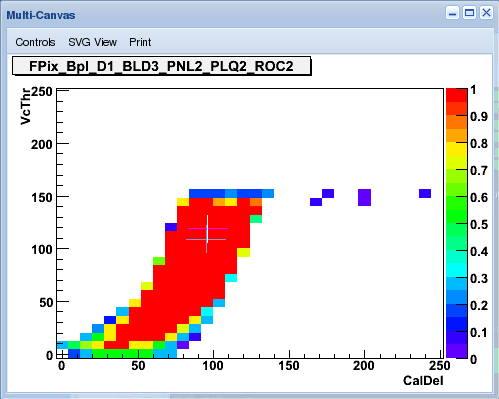
\includegraphics[width=0.8\linewidth]{VcThrCalDel_example.png}
\end{center}
\caption{The efficiency for detecting a hit is shown as a function of VcThr vs. CalDel. To large values of VcThr, corresponding to a low threshold, generates  much noise that saturates the digital circuit and no hits are seen. The optimal point is indicated in black and the blue point indicates the old point from the configuration. }
\label{fig:thresholdCalDel}
\end{figure}

\subsubsection{Results}
The primary output of this calibration are new ROC DAC settings. The only settings that should be changed in this calibration are for CalDel and VcThr.

\subsection{CalDelCalibation}

\subsubsection{Introduction}
Again the note from Sect.~\ref{sect:caldelvsvcthr} apply in that CalDel is not relevant for physics data.

In this calibration we scan CalDel for a series of different WBC settings. The creates a pattern as indicated in Fig.~\ref{fig:caldel}. As a change of one unit of WBC corresponds to  24.95ns (40.079 MHz) we can use the change in  CalDel for different WBC settings to calibrate absolutely what a change of CalDel corresponds to in absolute time. 

We run this calibration with an injection of a large signal (255 on the high Vcal range). We then pick a Vcal setting that is near the {\it early} start of the efficient range for the WBC setting. We pick an early time so that we retain efficiency for signals that are not as strong and takes time to get over  threshold. How close to the edge the CalDel setting  is taken can be specified by the parameter  ``Fraction''. Setting this to 0 means that you pick the point right at the early edge, setting the parameter to 1 means that you select the late edge. 

\subsubsection{Procedure}

\subsubsection{Parameters}
An example of a configuration file for the CalDel calibration is shown below:

\begin{verbatim}
Mode: CalDelCalibration
Rows:
10 | 20 
Cols:
10 | 20
VcalHigh
Scan: WBC 117 123 1
Scan: CalDel 0 255 1
Set: Vcal 250
Repeat: 2
ToCalibrate:
+ all
\end{verbatim}

If you want to just scan over WBC to find the right WBC value you can use a configuration that sets CalDel to a fixed value:

\begin{verbatim}
Mode: CalDelCalibration
Rows:
10 | 20
Cols:
10 | 20
VcalHigh
Scan: WBC 117 123 1
Scan: CalDel 100 100 1
Set: Vcal 250
Repeat: 2
ToCalibrate:
+ all
\end{verbatim}

\subsubsection{Output}
The calibration also generates output to display the region of good  efficiency in the WBC vs CalDel. The output can be processed to generate plots using the root script {\tt caldel.c}. An example plot is shown in  Fig.~\ref{fig:caldel}

\begin{figure}
\begin{center}
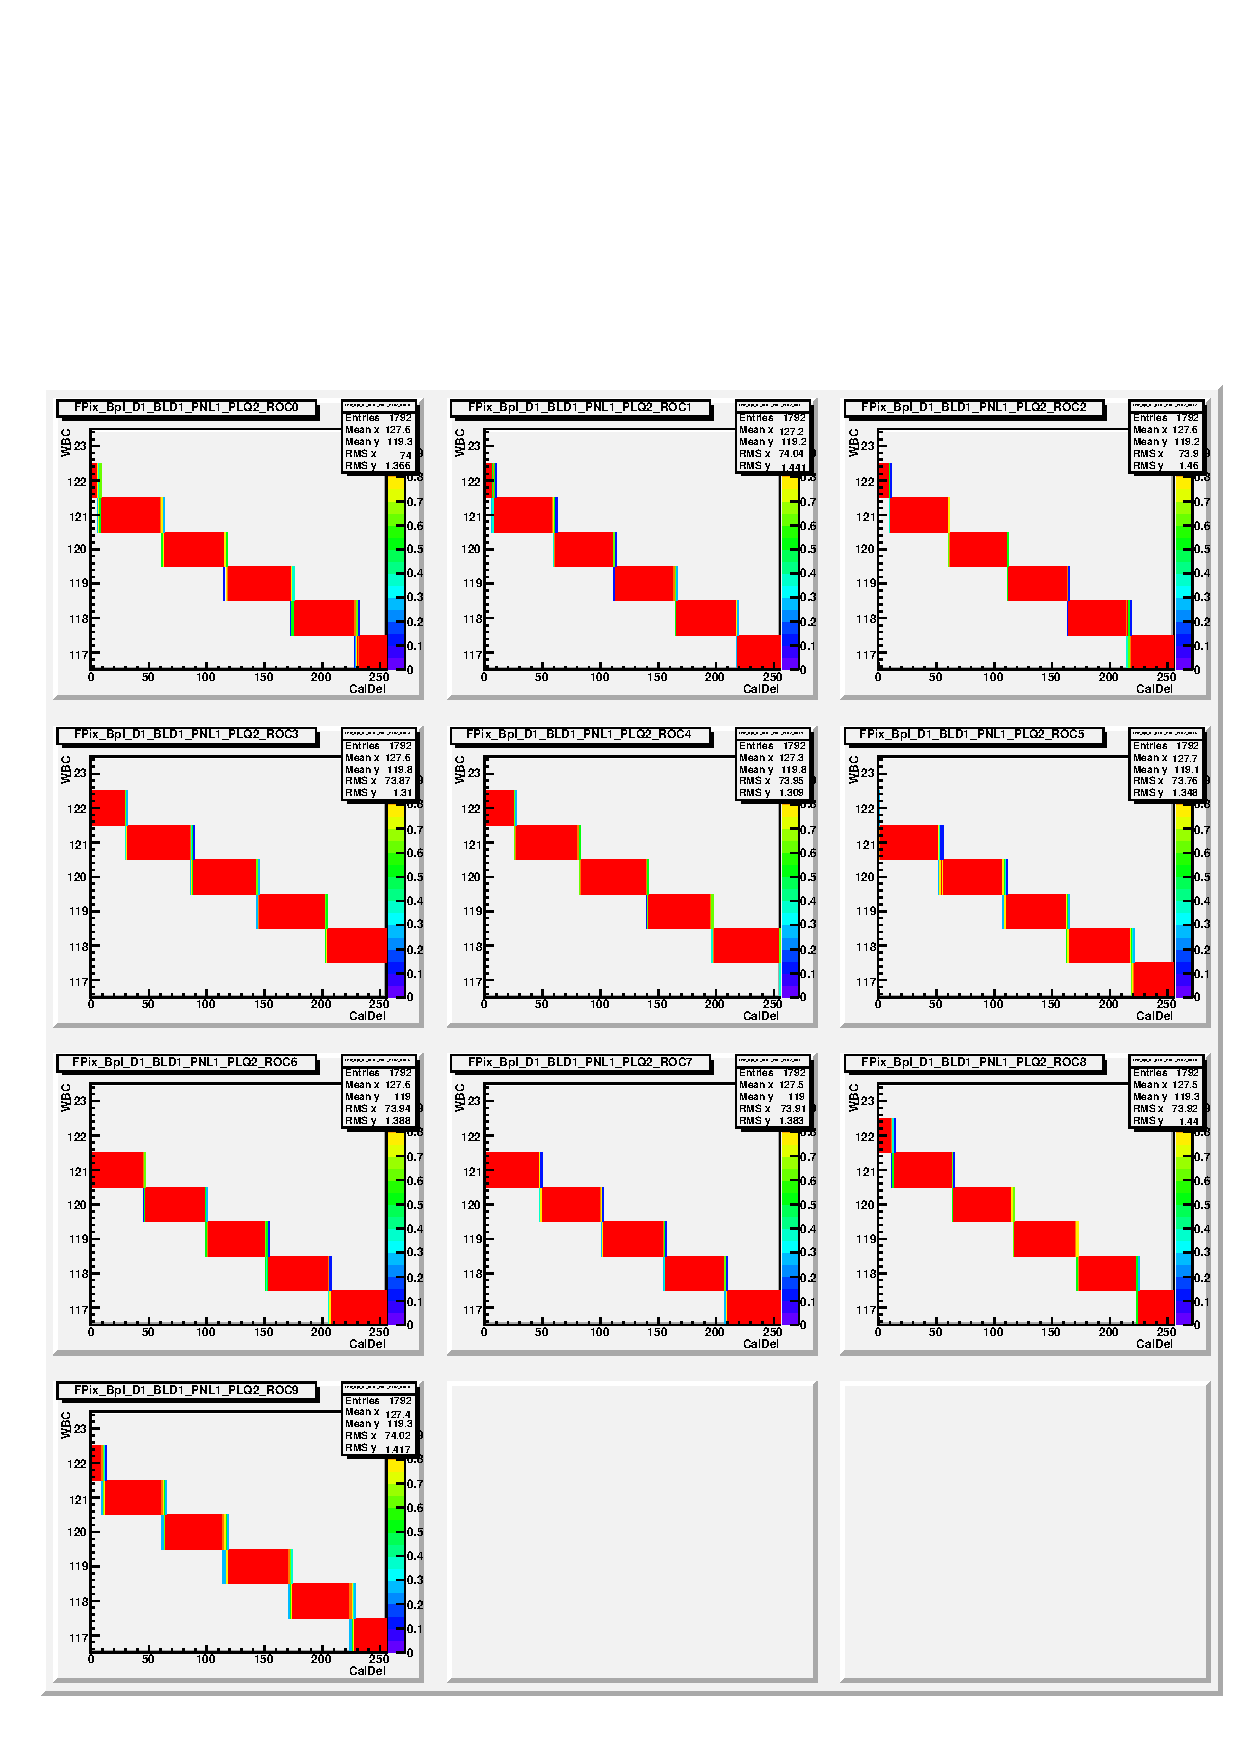
\includegraphics[width=\linewidth]{CalDelCalibration}
\end{center}
\caption{
The efficiency as a function of WBC vs CalDel.
}
\label{fig:caldel}
\end{figure}

\subsubsection{Results}
The CalDel calibration produces new ROC DAC settings that update the CalDel settings, all other settings should be left unchanged.

%\subsection{Idigi vs. Vsf}

%In this 'calibration' we scan Vsf and measure the digital current. This is not really a calibration as we don't determine any settings from this. Rather what we do is to find a maximum Vsf setting that we will use. If Vsf is too large the digital current increases. In the configuration for this calibration you can set the maximum increase in Idigi that you allow using the parameter IdigiMax (units are in mA). {\it Not yet implemented, there is a hardcoded number of 7 mA now.}

%\subsubsection{Example}

%The configuration used for the digital scan
%looks like
%\begin{verbatim}
%Mode:  Idigi
%Rows:
%Cols:
%Vcal:
%200 200 5
%Repeat:
%1
%ToCalibrate:
%+ all
%\end{verbatim}

%\subsubsection{Output}

%This calibration produces the object  PixelMaxVsf which is used in the calibration that determines Vsf to optimize the linearity.  In addition this calibration produces output  in a file called idigi.dat. Using the root script idigi.c you can generate plots as  shown in Fig.~\ref{fig:IdigivsVsf}.

%\begin{figure}
%\begin{center}
%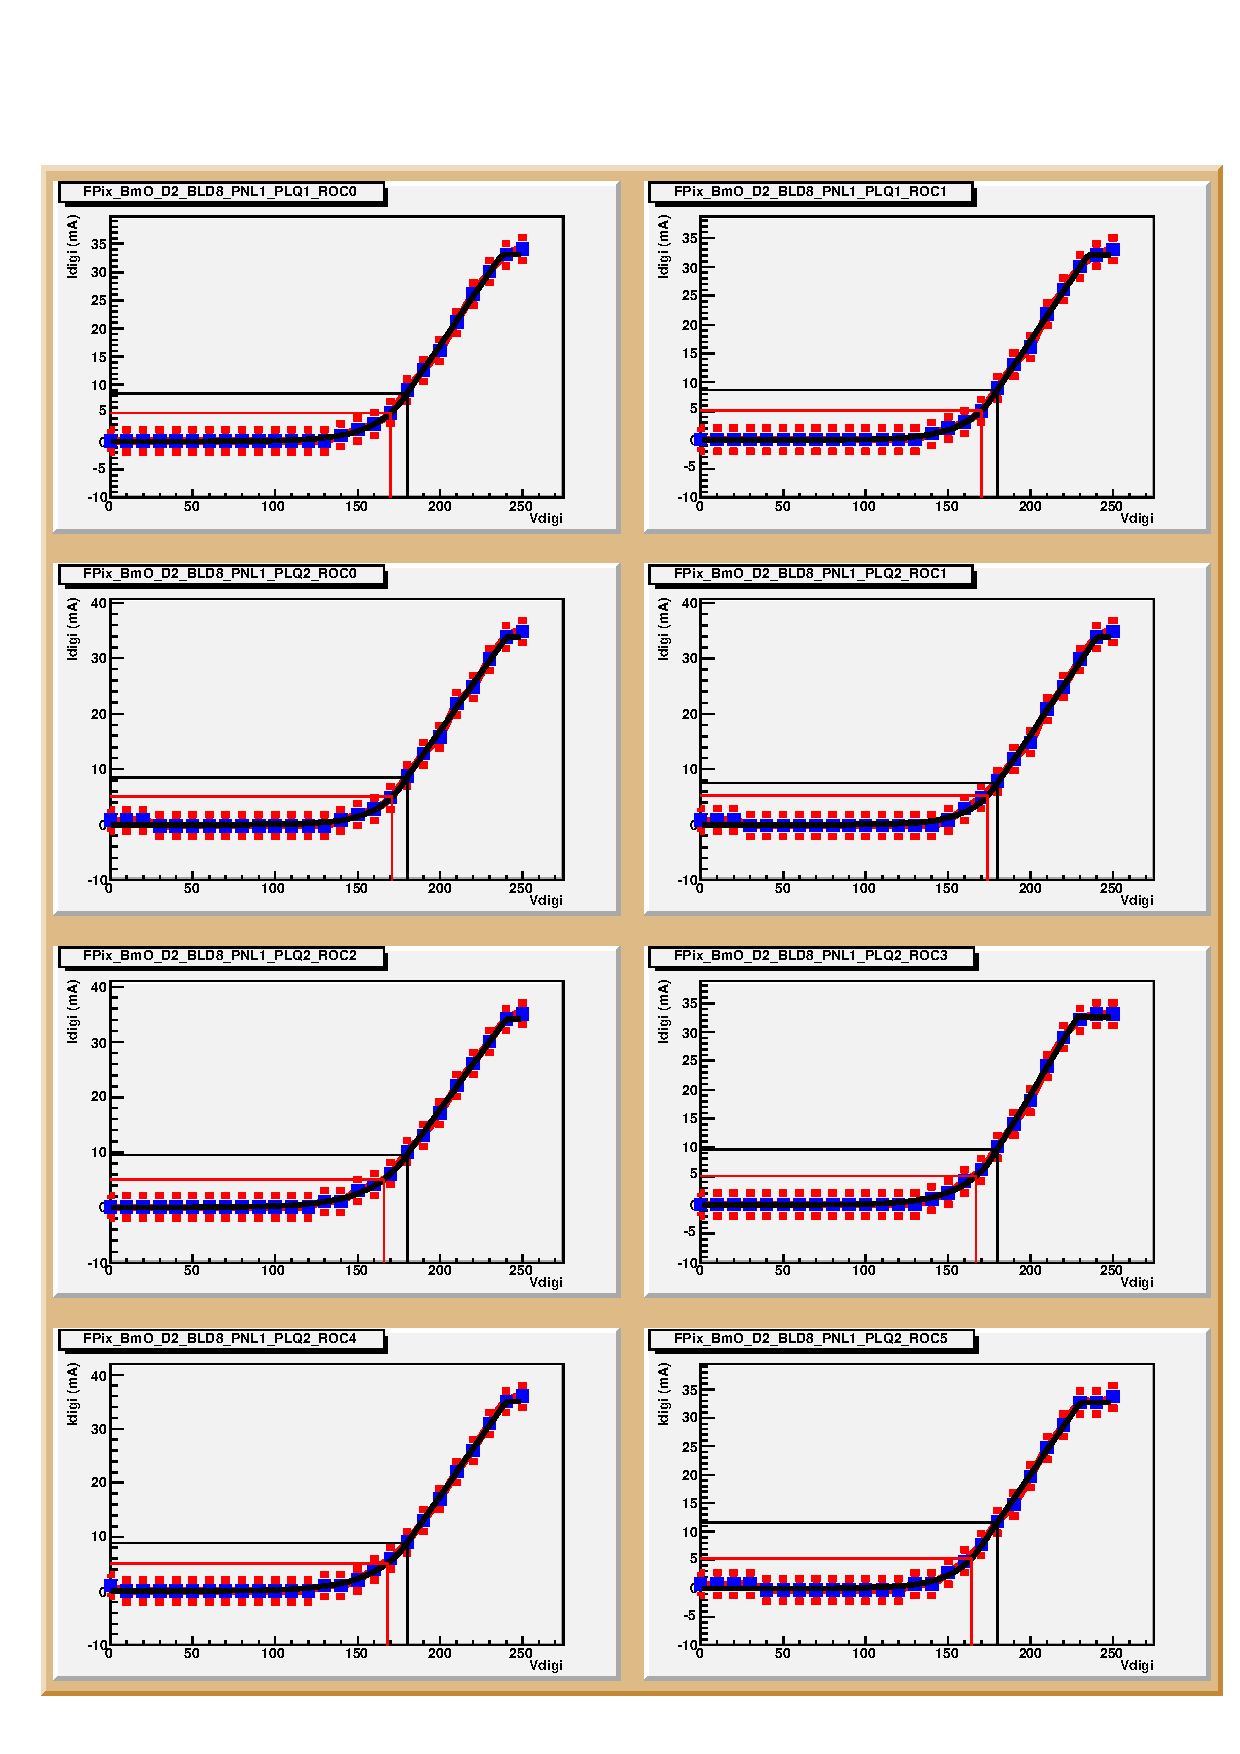
\includegraphics[width=\linewidth]{idigi1}
%\end{center}
%\caption{The digital current is shown as a function of Vsf. }
%\label{fig:IdigivsVsf}
%\end{figure}


\subsection{Linearity vs.~Vsf}
\label{sec:LinearityVsVsf}

The ROC DAC setting \verb|Vsf| affects the linearity of the pixel response vs.~received charge; larger values improve linearity.  \verb|Vsf| also affects the digital current, with higher values increasing the current.  We have implemented two algorithms to set \verb|Vsf| at a value that gives good linearity without drawing excessive power.  The first, described in this section, is the algorithm developed at PSI.

\subsubsection{Introduction and discussion}

This algorithm measures linearity from scans of pulse height vs.~\verb|Vcal| at different values of \verb|Vsf|.  Examples of these scans are shown in Fig.~\ref{fig:PH_vs_Vcal_scans}.

\begin{figure}
\begin{center}
 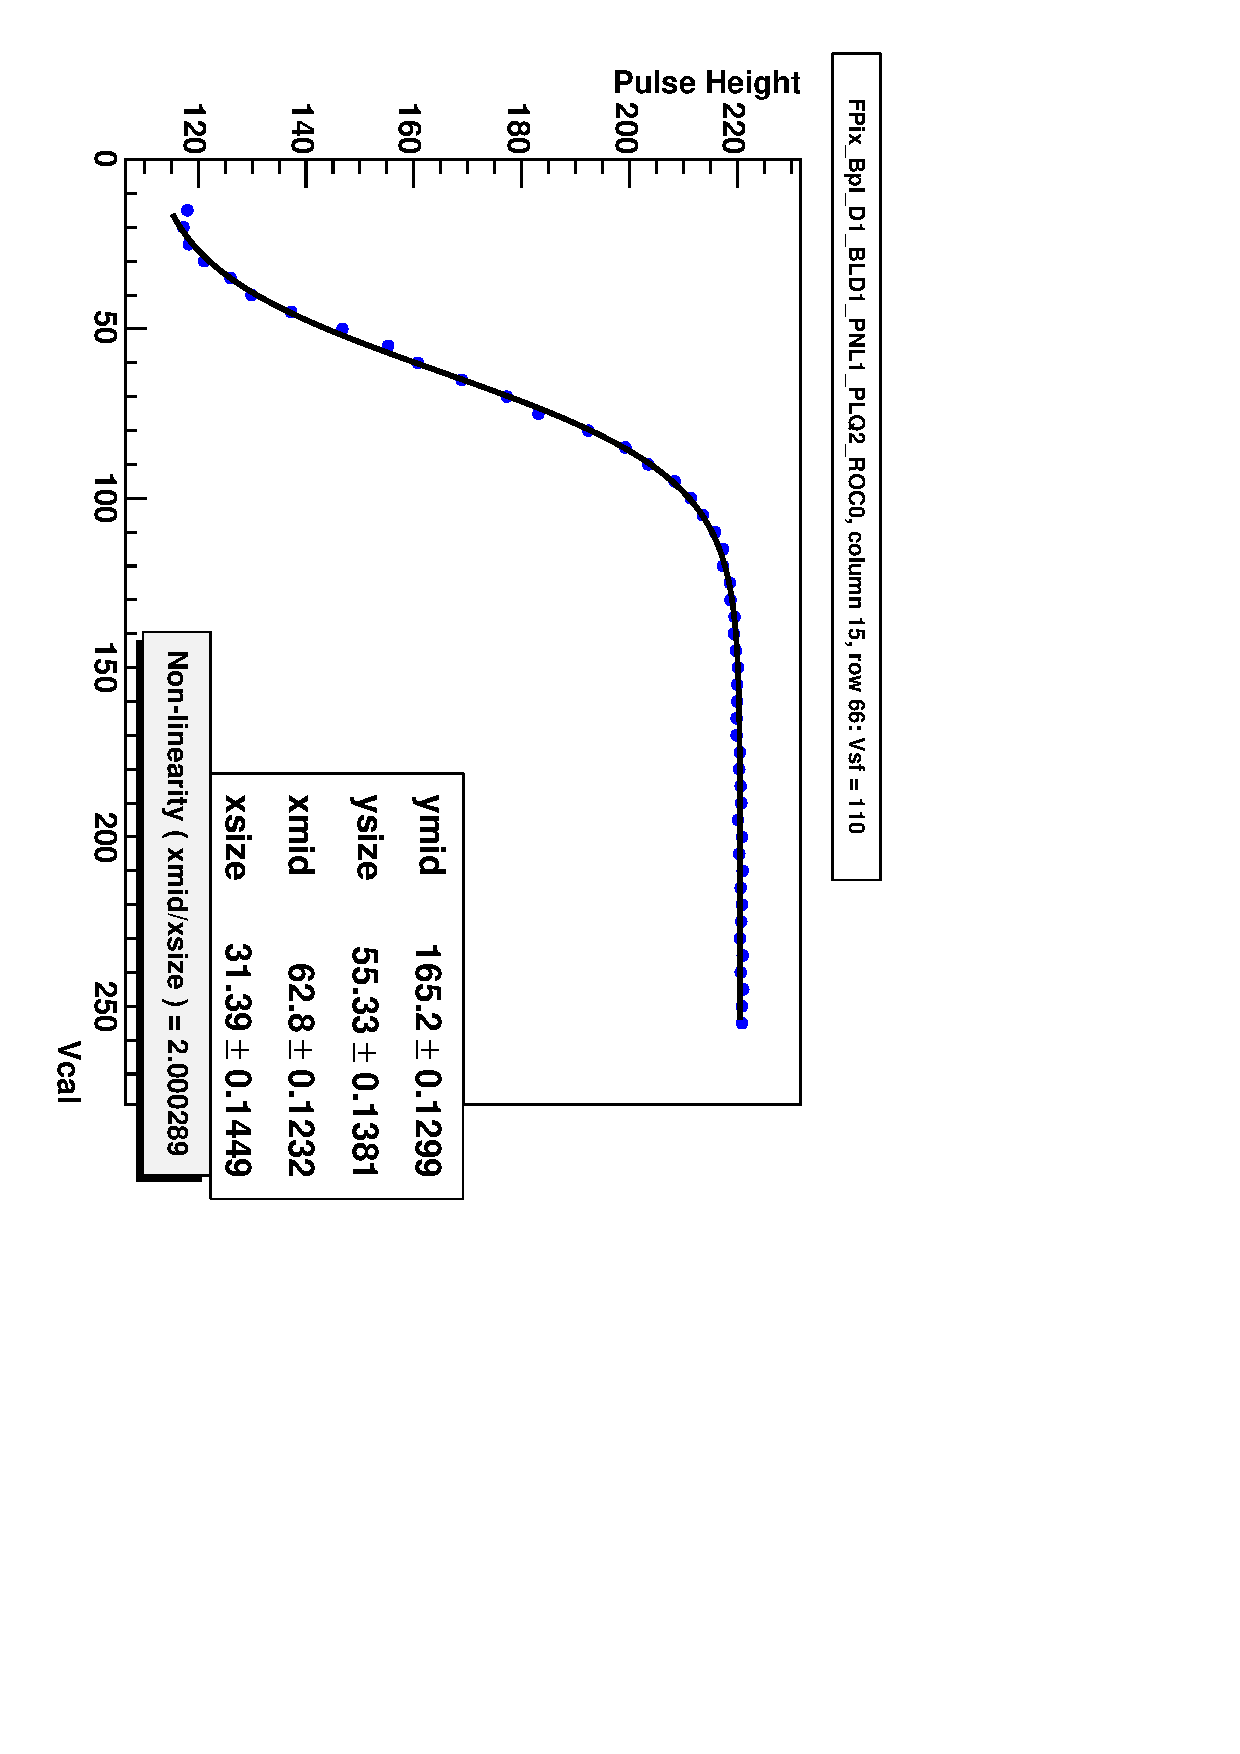
\includegraphics[angle=90,width=0.49\textwidth]{PH_vs_Vcal_poorLinearity.pdf}
 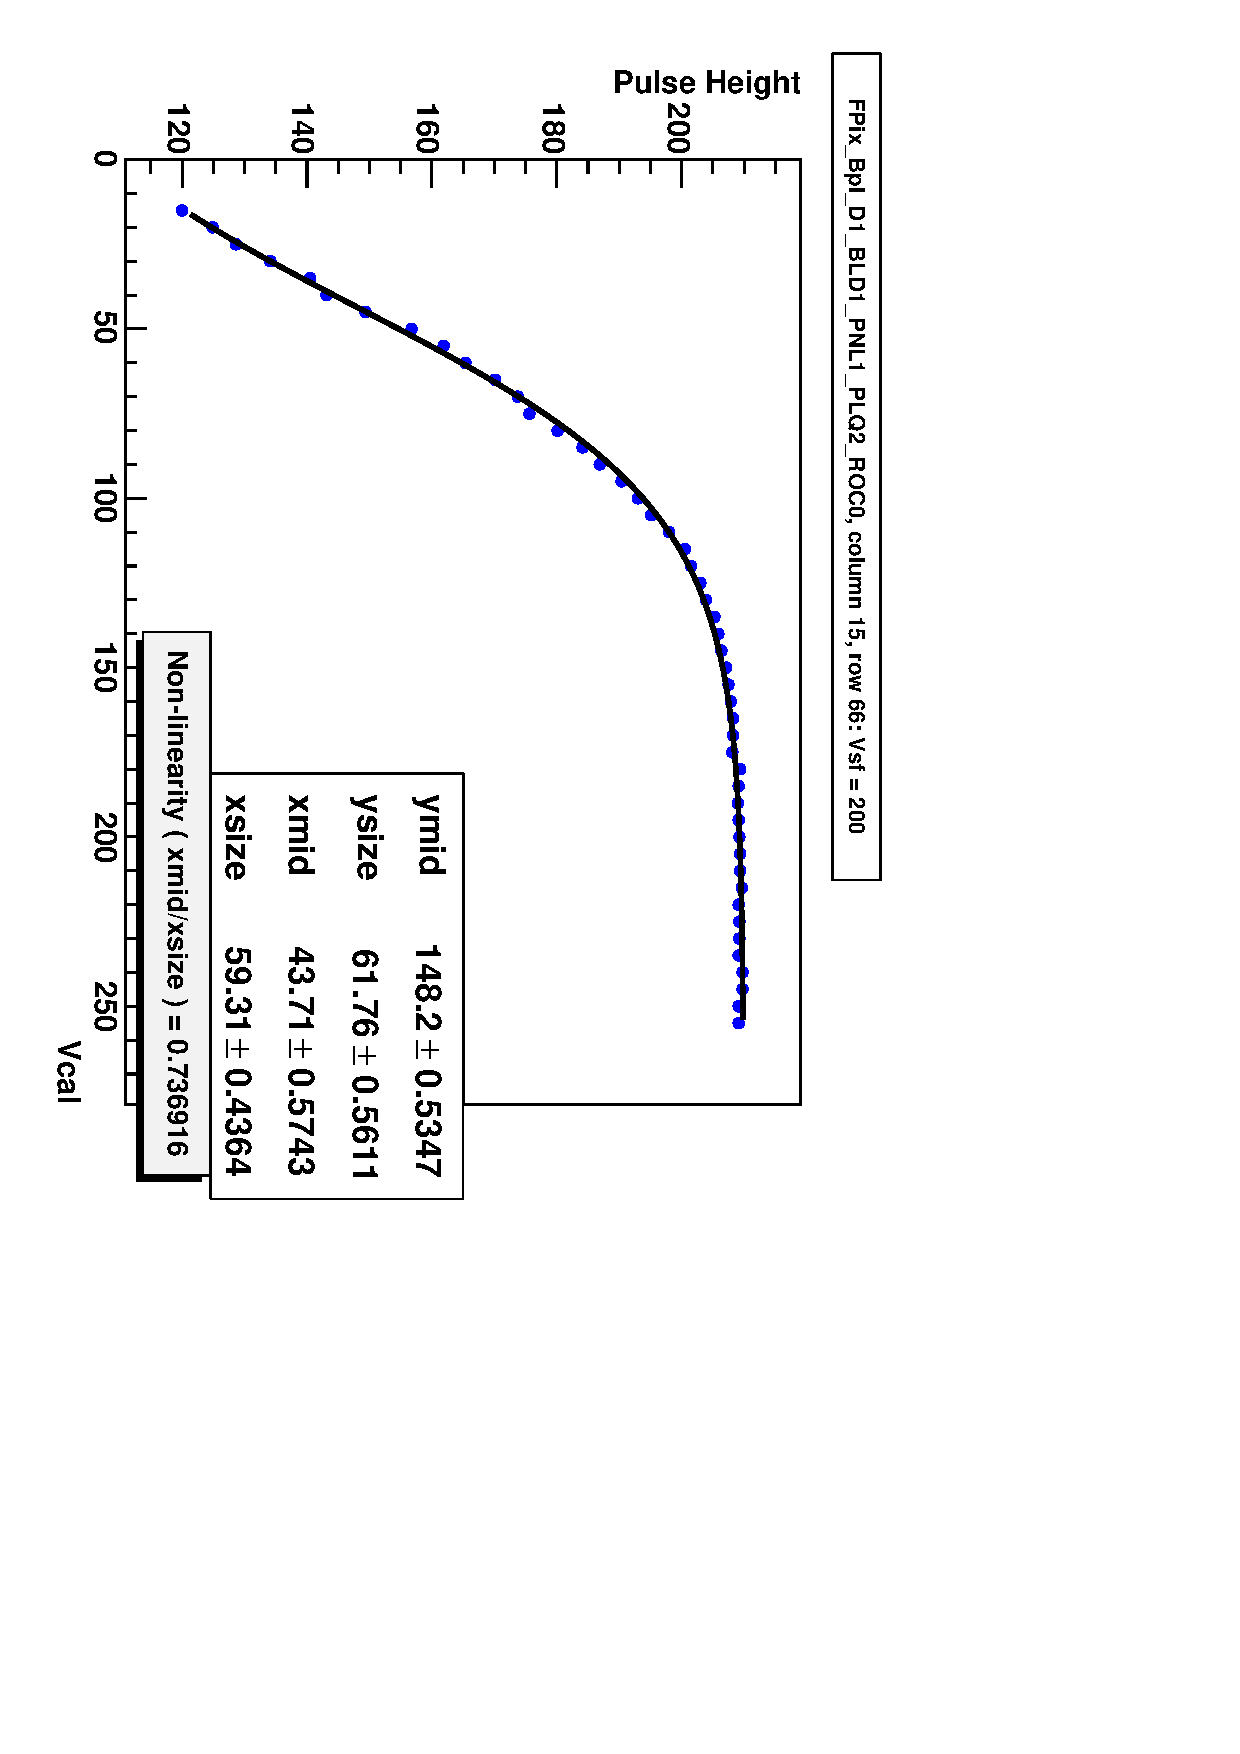
\includegraphics[angle=90,width=0.49\textwidth]{PH_vs_Vcal_goodLinearity.pdf}
\end{center}
\caption{Scans of pulse height vs.~Vcal at different values of Vsf.  The scan on the left has poor linearity, and the scan on the right has good linearity.  (Note that these scans come from a detector which has no voltage bias, so the received charge and the slope of the linear section are lower than in a biased detector.)}
\label{fig:PH_vs_Vcal_scans}
\end{figure}

To quantify the degree of nonlinearity, the scan data are fit with a function
\begin{equation} \label{eq:tanh}
PH = f(Vcal) = y_{\rm mid} + y_{\rm size} \times \tanh \left( \frac{Vcal - x_{\rm mid}}{x_{\rm size}} \right)
\end{equation}
where $PH$ is the recorded pulse height, $Vcal$ is the input, $(x_{\rm mid},y_{\rm mid})$ is the point at the center of the quasi-linear rise region of the hyperbolic tangent, $x_{\rm size}$ is the horizontal scale of the quasi-linear region, and $y_{\rm size}$ is the vertical scale of that region.

From this fit, the degree of nonlinearity can be quantified in different ways.  The simpler nonlinearity parameter, used by PSI and used by default in this calibration, is $x_{\rm mid}/x_{\rm size}$.  When this parameter is small, it means that \verb|Vcal| = 0 lies within the quasi-linear rise region, and hence the response is linear for small amounts of injected charge.  PSI has used $x_{\rm mid}/x_{\rm size} = 1.4$ as the cutoff -- values below 1.4 indicate good linearity.

An alternate nonlinearity parameter is
\begin{equation} \label{eq:nonlinearityIntegral}
\frac{1}{2} \int_{Vcal_{\rm min}}^{Vcal_{\rm max}} dVcal \left| \frac{f''(Vcal)}{f'(Vcal)} \right|
\end{equation}
where $f(Vcal)$ is the hyperbolic tangent function in Eq.~(\ref{eq:tanh}).  This integral is a measure of the vertical change due to curvature divided by the vertical change due to slope over the range of the integral.  The limits of the integral should be chosen to include the range for which we want good linearity.  By default the limits go from \verb|Vcal| = 50 to \verb|Vcal| = 400 in low-scale \verb|Vcal| units, or from 50/7 to 400/7 in high-scale units.  This integral can be evaluated analytically.

Figure~\ref{fig:nonlinearityPlots} shows scans of both measures of nonlinearity vs.~\verb|Vsf|.  As seen in the plots, they give similar shapes.  This calibration allows the user to use either measure; the default is $x_{\rm mid}/x_{\rm size}$.

\begin{figure}
\begin{center}
 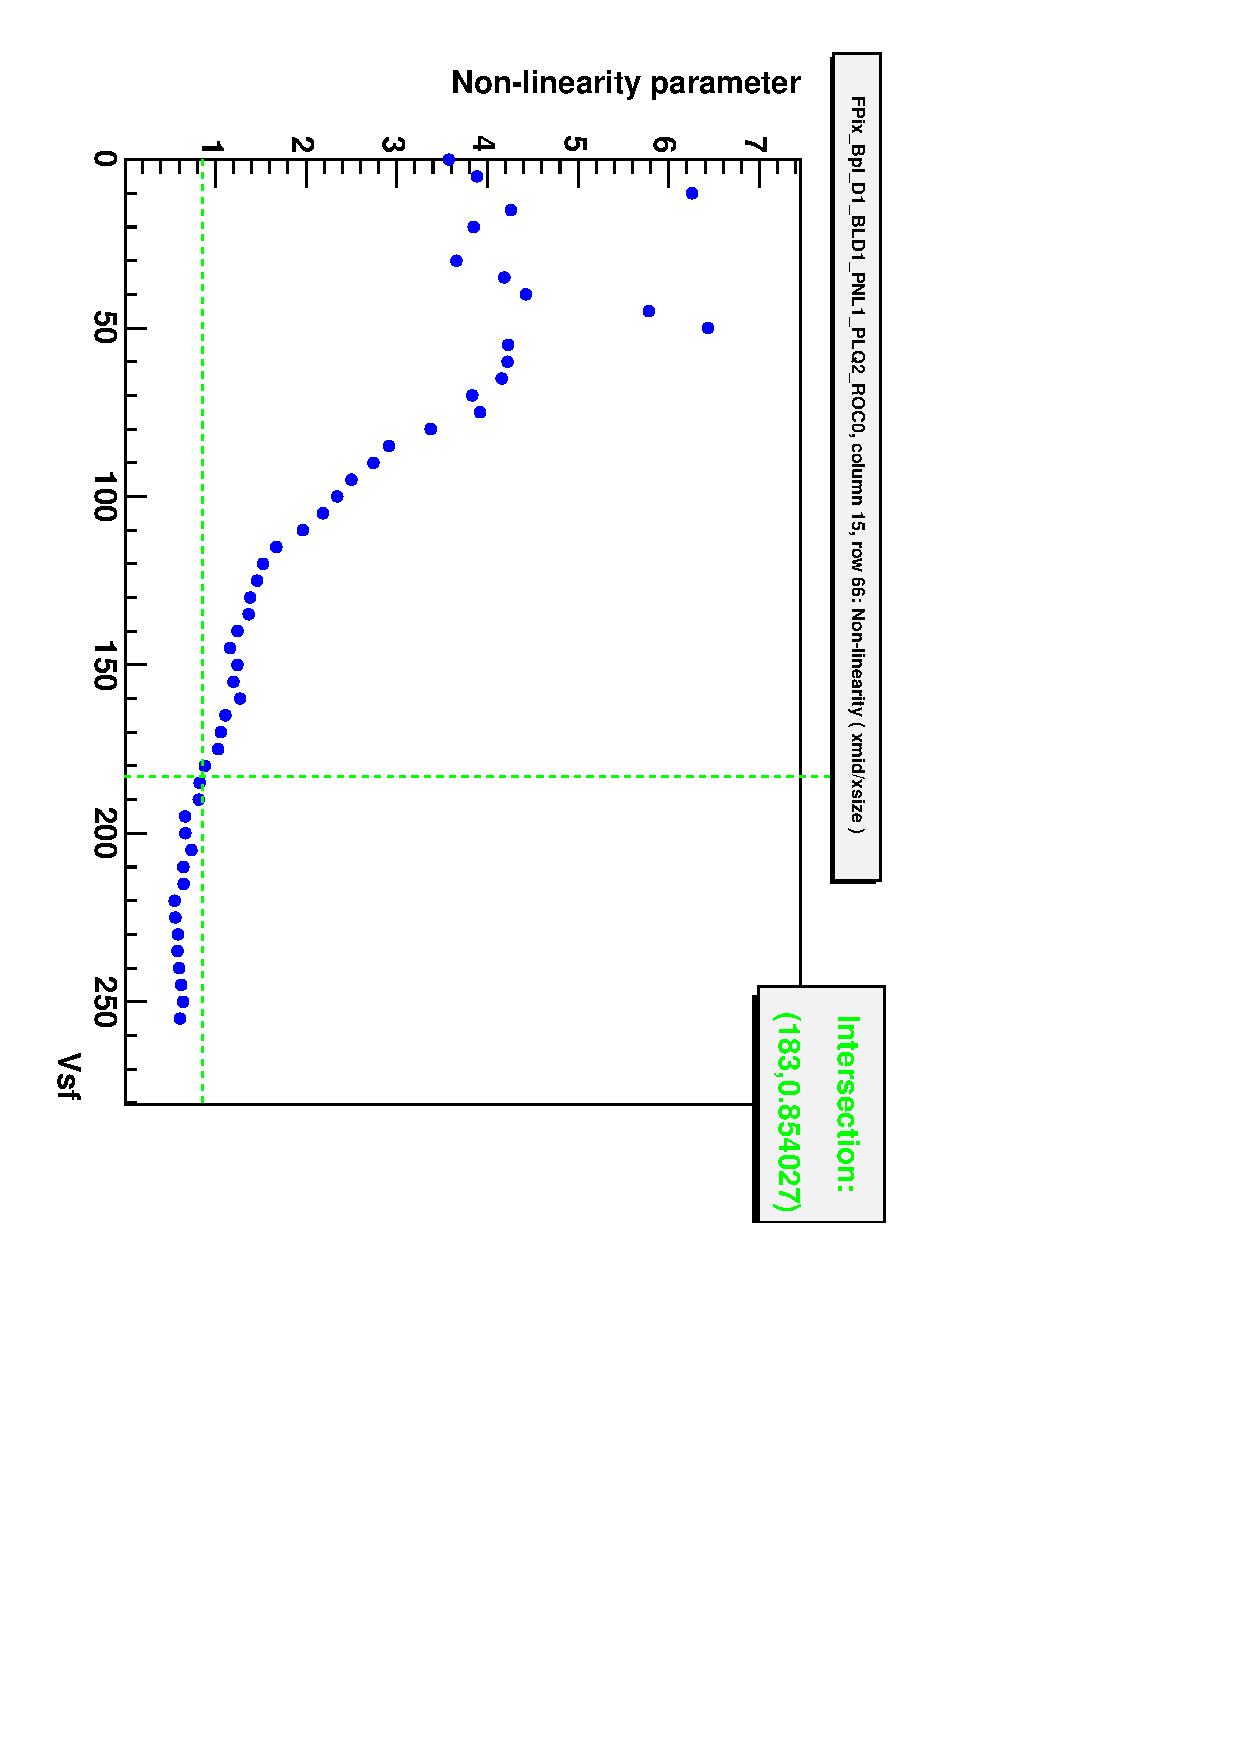
\includegraphics[angle=90,width=0.49\textwidth]{nonlinearityPlot_xmidOverXsize.pdf}
 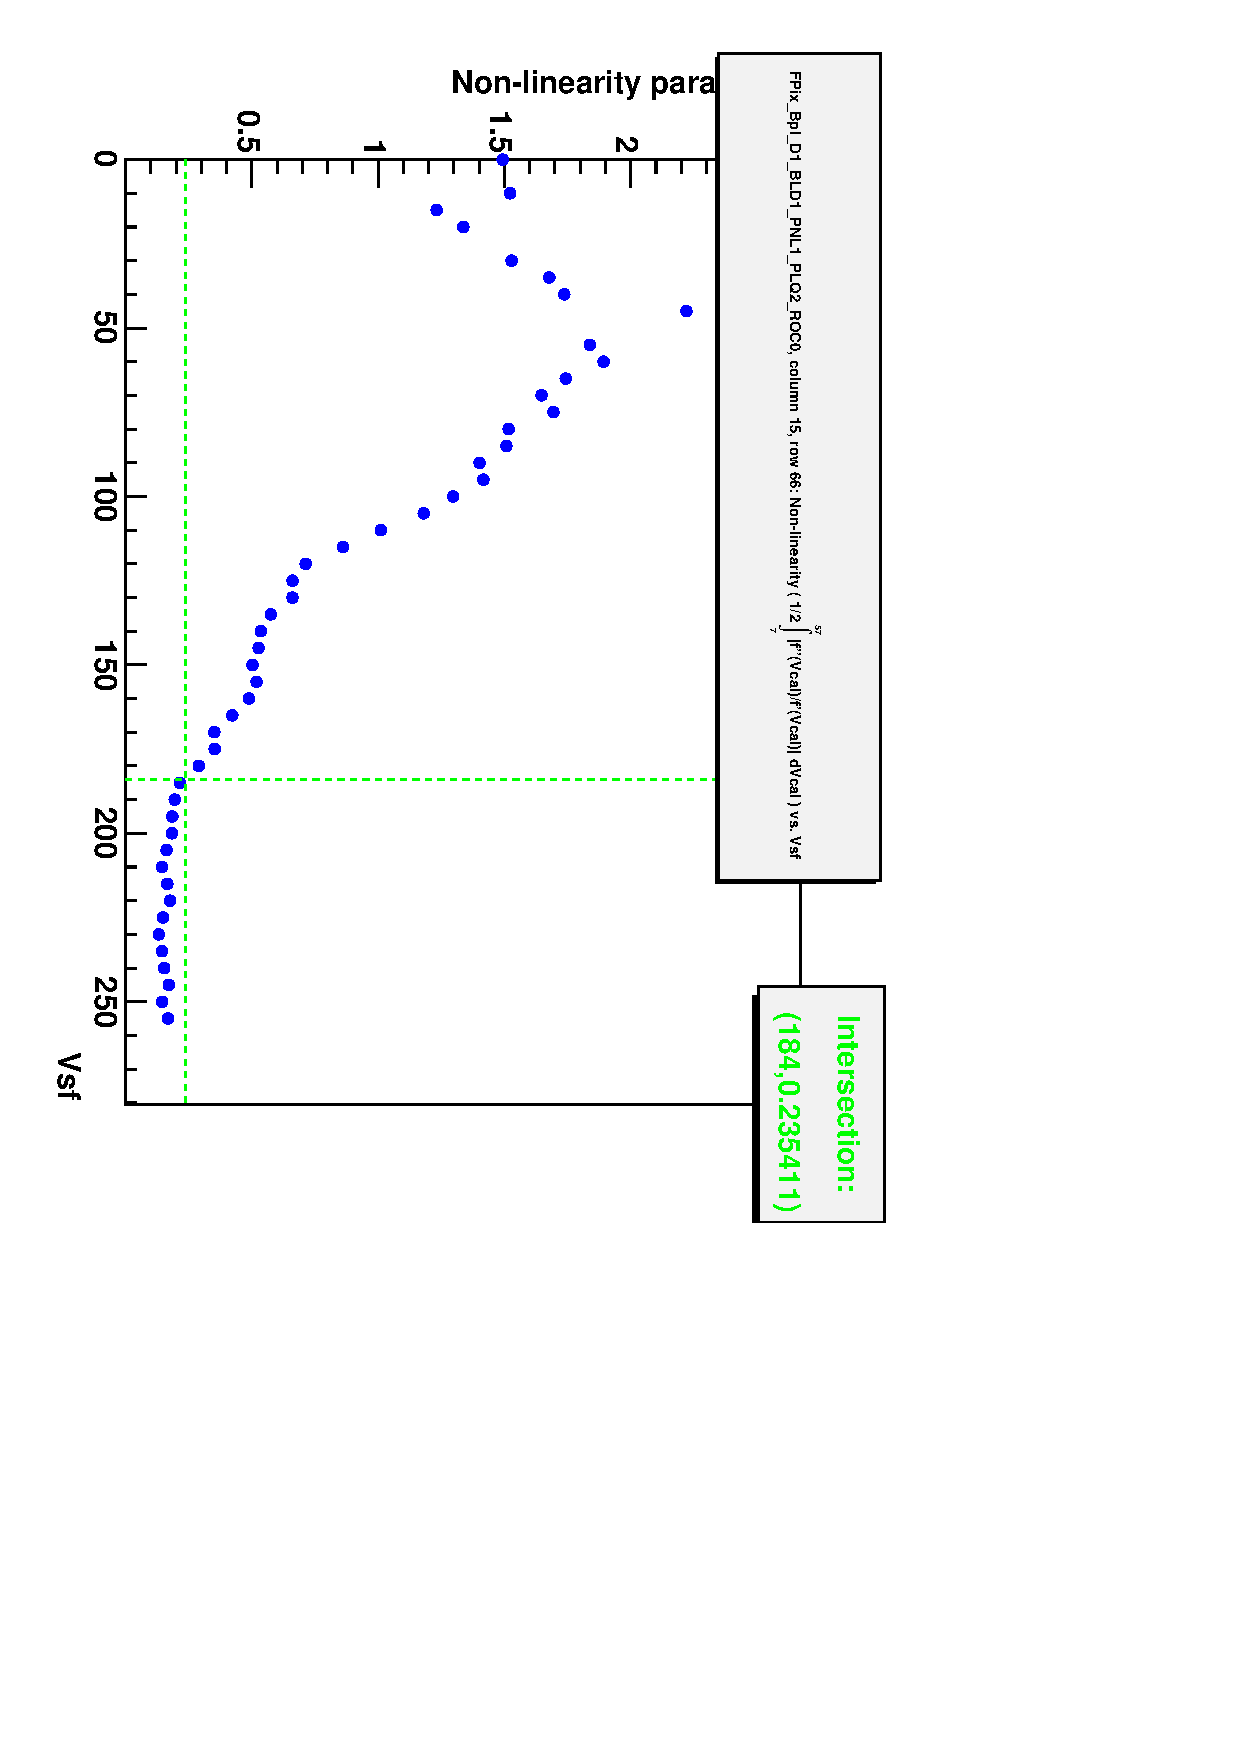
\includegraphics[angle=90,width=0.49\textwidth]{nonlinearityPlot_integral.pdf}
\end{center}
\caption{Plots of nonlinearity vs.~Vsf.  On the left, nonlinearity is measured by $x_{\rm mid}/x_{\rm size}$, and on the right, it is measured by the integral in Eq.~(\ref{eq:nonlinearityIntegral}).}
\label{fig:nonlinearityPlots}
\end{figure}

\subsubsection{Linearity vs.~Vsf calibration steps}

This calibration consists of the following steps:
\begin{enumerate}
\item Scan \verb|Vcal| and \verb|Vsf| according to the calibration's configuration.  On each trigger, read out data from each FED's FIFO3.  Record the pulse height, keeping separate scans for different pixels.
\item For each scan of pulse height vs.~\verb|Vcal| (for a given ROC, pixel, and \verb|Vsf| value), fit with the function in Eq.~(\ref{eq:tanh}).  A plot of each scan and fit is written to a ROOT file (see Fig.~\ref{fig:PH_vs_Vcal_scans}).  If the fit is successful, compute the nonlinearity parameter (either $x_{\rm mid}/x_{\rm size}$ or the integral in Eq.~(\ref{eq:nonlinearityIntegral})) and add it to a scan of nonlinearity vs.~\verb|Vsf| for that ROC and pixel.  This scan is also written to a ROOT file (see Fig.~\ref{fig:nonlinearityPlots}).
\item For each scan of nonlinearity vs.~\verb|Vsf|, determine an optimal \verb|Vsf|.  This is done by finding the highest \verb|Vsf| where the scan intersects a nonlinearity threshold.  This threshold may be either absolute or relative, according to the parameter ``\verb|absoluteNonlinearityThreshold|".  If absolute, the threshold is set by the parameter ``\verb|nonlinearityThreshold|".  If relative, the threshold is the value of the nonlinearity at the highest \verb|Vsf| in the scan, multiplied by the parameter ``\verb|nonlinearityThreshold|".
\item For each ROC, examine the optimal \verb|Vsf|s on the various pixels.  If there are at least 4 pixels, discard any \verb|Vsf| outliers.  After any discarding, average the \verb|Vsf| values to determine the \verb|Vsf| setting for that ROC.
\item Compare the \verb|Vsf| setting on each ROC to the maxVsf setting in the configuration.  If the setting from this calibration exceeds the maximum, reduce \verb|Vsf| to the maximum allowed.
\item Write out new ROC configuration files for the successfully-calibrated
ROCs with the new \verb|Vsf| settings.
\item Print out a summary.
\end{enumerate}

\subsubsection{Parameters}
A number of parameters in \verb|calib.dat| may be used to control the
calibration.

The various ``standard" parameters are used in this calibration.  The
``\verb|Repeat:|" parameter determines the number of triggers in each step
of the scan.  The ROC list is used to determine which ROCs are calibrated.

The scan ranges are specified by lines like
\begin{verbatim}
Scan: Vcal  0 255 5
Scan: Vsf   0 255 5 mix
\end{verbatim}
which specify the scan range and step size.  The ``\verb|mix|'' flag must be enabled for \verb|Vsf| (or alternatively SingleROC mode must be used); otherwise the calibration will abort.

The hits specified in \verb|Rows:| and \verb|Columns:| will be
used.  One scan is taken for each pixel with hits.  At most two hits per pixel pattern may be specified (or alternatively SingleROC mode must be used); otherwise the calibration will abort.  The reason for this restriction is that the FED's spy FIFO3 will overflow if each ROC connected to it has more than two hits.

Some optional parameters may also be set.  All have default values which will
be used if the parameter is not set.  These parameters, their defaults, and
their functionality are given in Table~\ref{tab:LinearityVsVsfParameters}.

\begin{table}
\centering
\caption{Optional parameters for linearity vs. Vsf calibration.}
\label{tab:LinearityVsVsfParameters}
\begin{tabular}{l@{~~~~}l@{~~~~}l}
\hline
\hline
Parameter & Default & Description \\
\hline
absoluteNonlinearityThreshold     & yes   & Whether the nonlinearity threshold is an \\
                                  &       &   absolute number, or a multiple of the \\
                                  &       &   nonlinearity parameter at maximum \verb|Vsf| \\
nonlinearityThreshold             & 1.4   & Value of the nonlinearity threshold \\
useIntegrated2ndOver1stDerivative & no    & Whether to use the integral in Eq.~(\ref{eq:nonlinearityIntegral}) for the \\
                                  &       &   nonlinearity parameter, instead of $x_{\rm mid}/x_{\rm size}$ \\
integralMinVcal                   &  50/7 & Lower \verb|Vcal| bound of the integral (if used) \\
integralMaxVcal                   & 400/7 & Upper \verb|Vcal| bound of the integral (if used) \\
\hline
\hline
\end{tabular}
\end{table}

\subsection{Vsf and VHldDel}

\subsubsection{Introduction and discussion}

We have also implemented the Renaissance algorithm for determining the ROC DAC settings \verb|Vsf| and \verb|VHldDel|.  Figure~\ref{fig:PHvsVHldDel} shows plots of pulse height vs.~\verb|VHldDel| at low, medium, and high values of \verb|Vsf|, with \verb|Vcal| = 250 on the low scale.  A good \verb|Vsf| value is one for which this curve rises and then falls so that the pulse heights at the two endpoints (lowest and highest \verb|VHldDel|) are equal.  Figure~\ref{fig:PHvsVHldDel} also includes a plot of these endpoints as a function of \verb|Vsf|; the rightmost intersection point is the \verb|Vsf| value chosen.  Low values of \verb|Vsf|, below $\sim$90, produce garbage output.

\begin{figure}
\begin{center}
 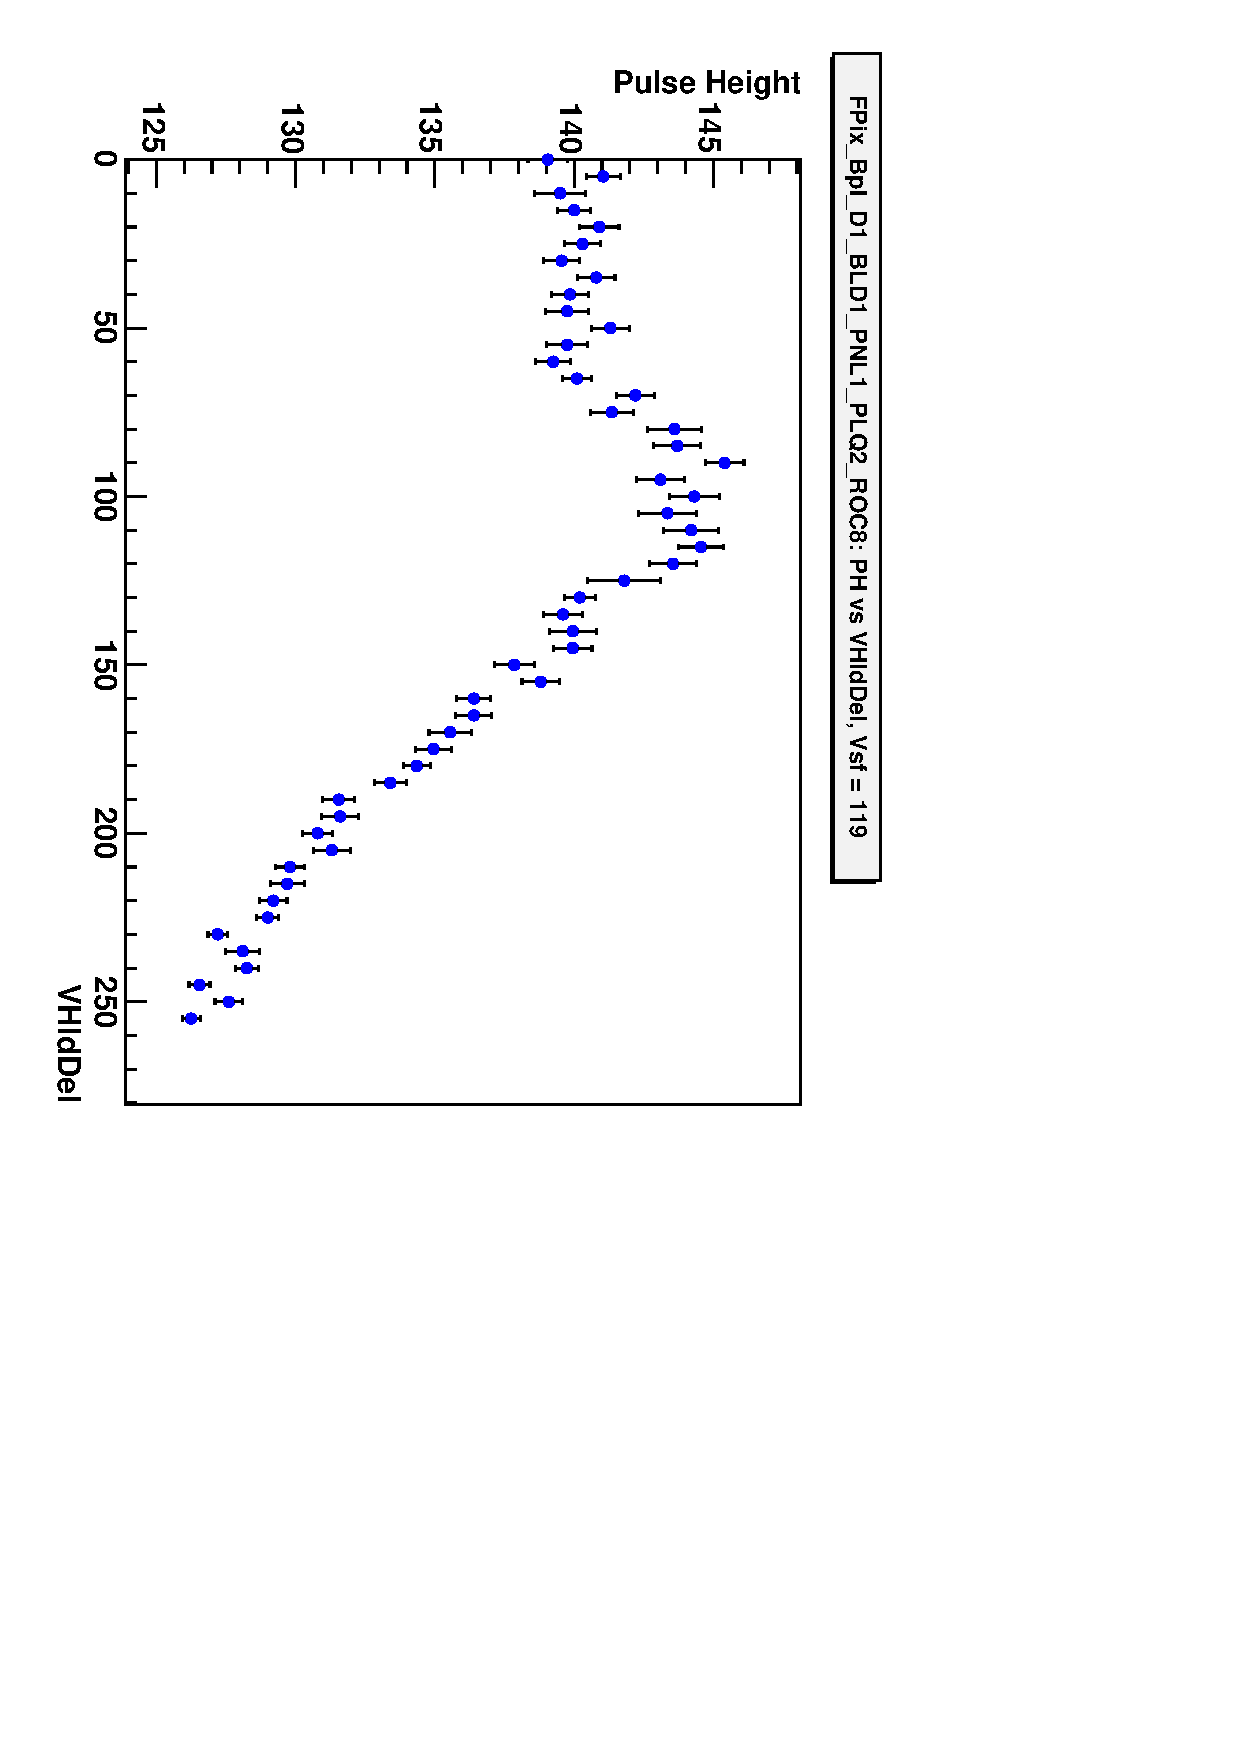
\includegraphics[angle=90,width=0.32\textwidth]{PH_vs_VHldDel_Vsf119.pdf}
 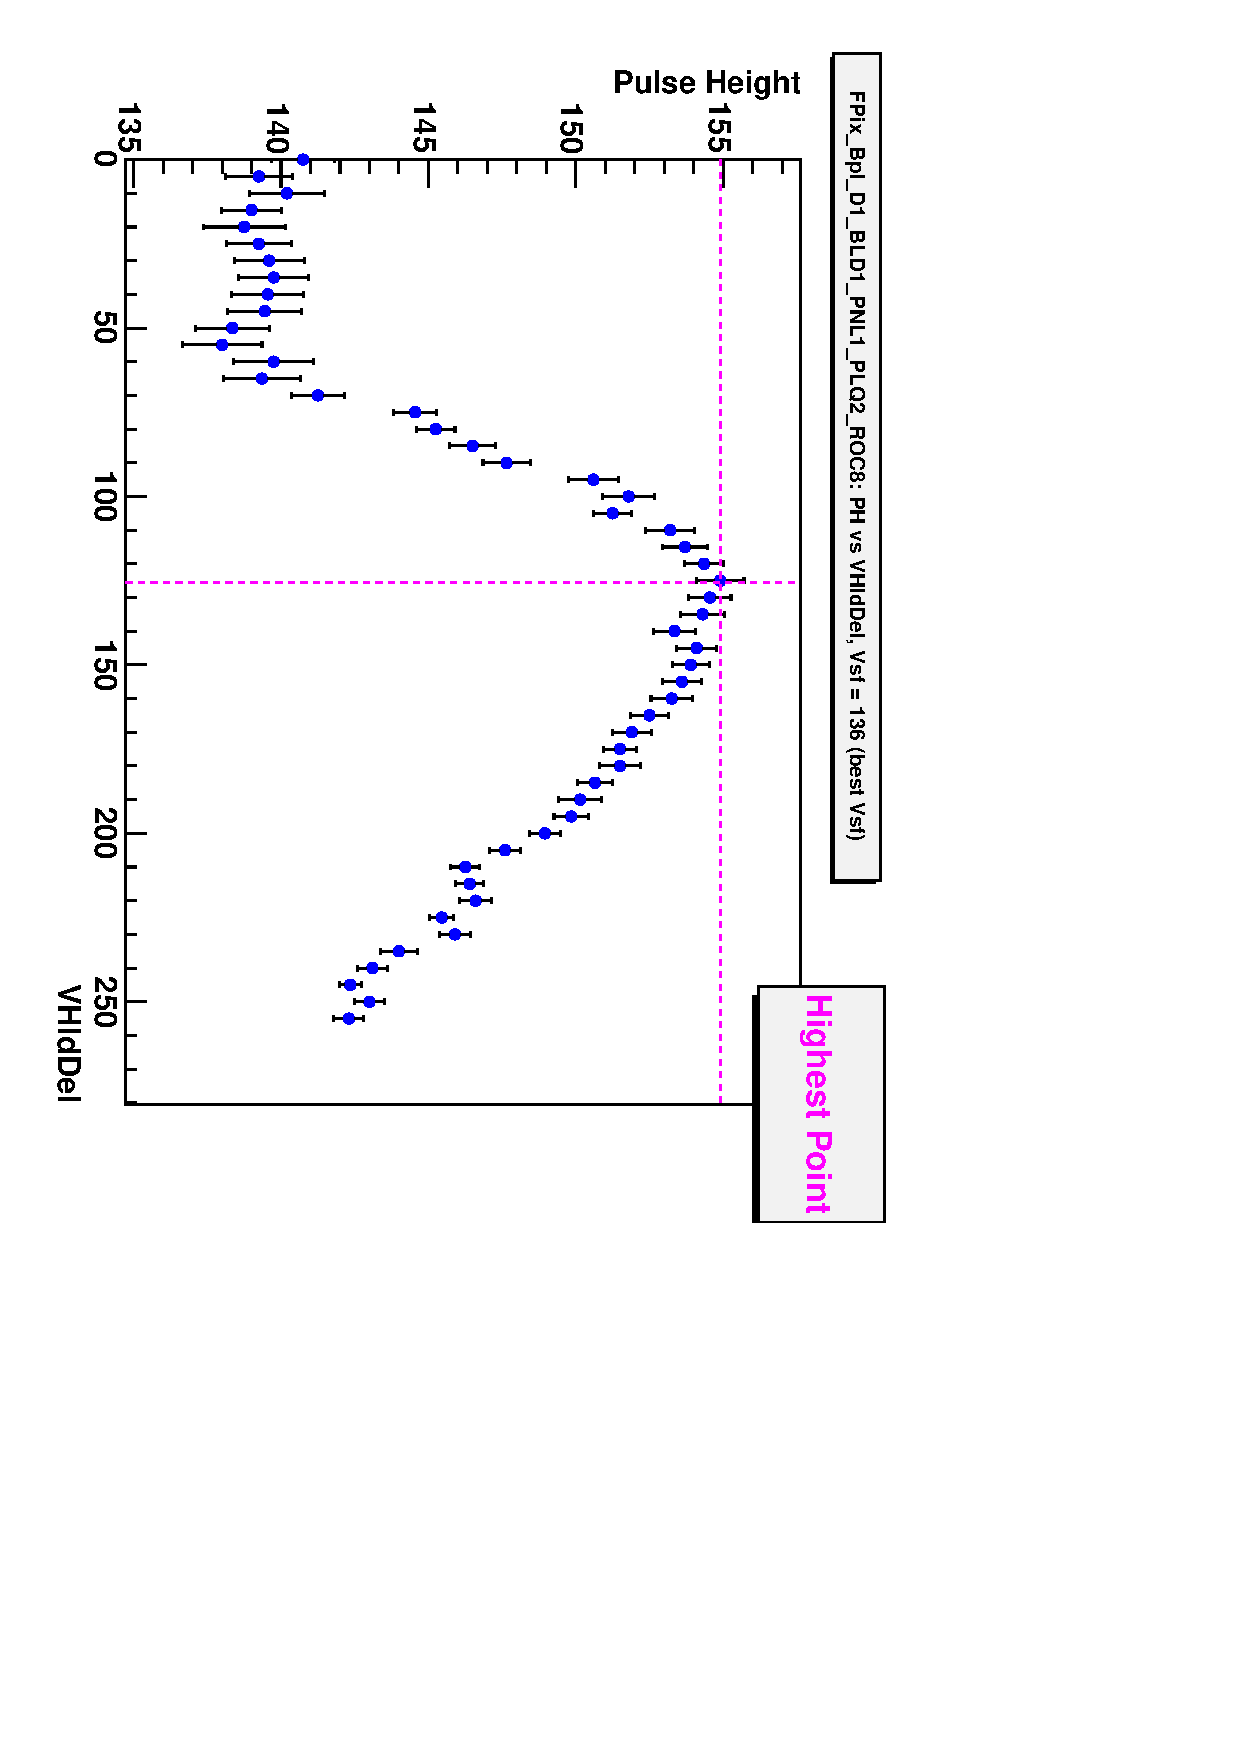
\includegraphics[angle=90,width=0.32\textwidth]{PH_vs_VHldDel_Vsf136.pdf}
 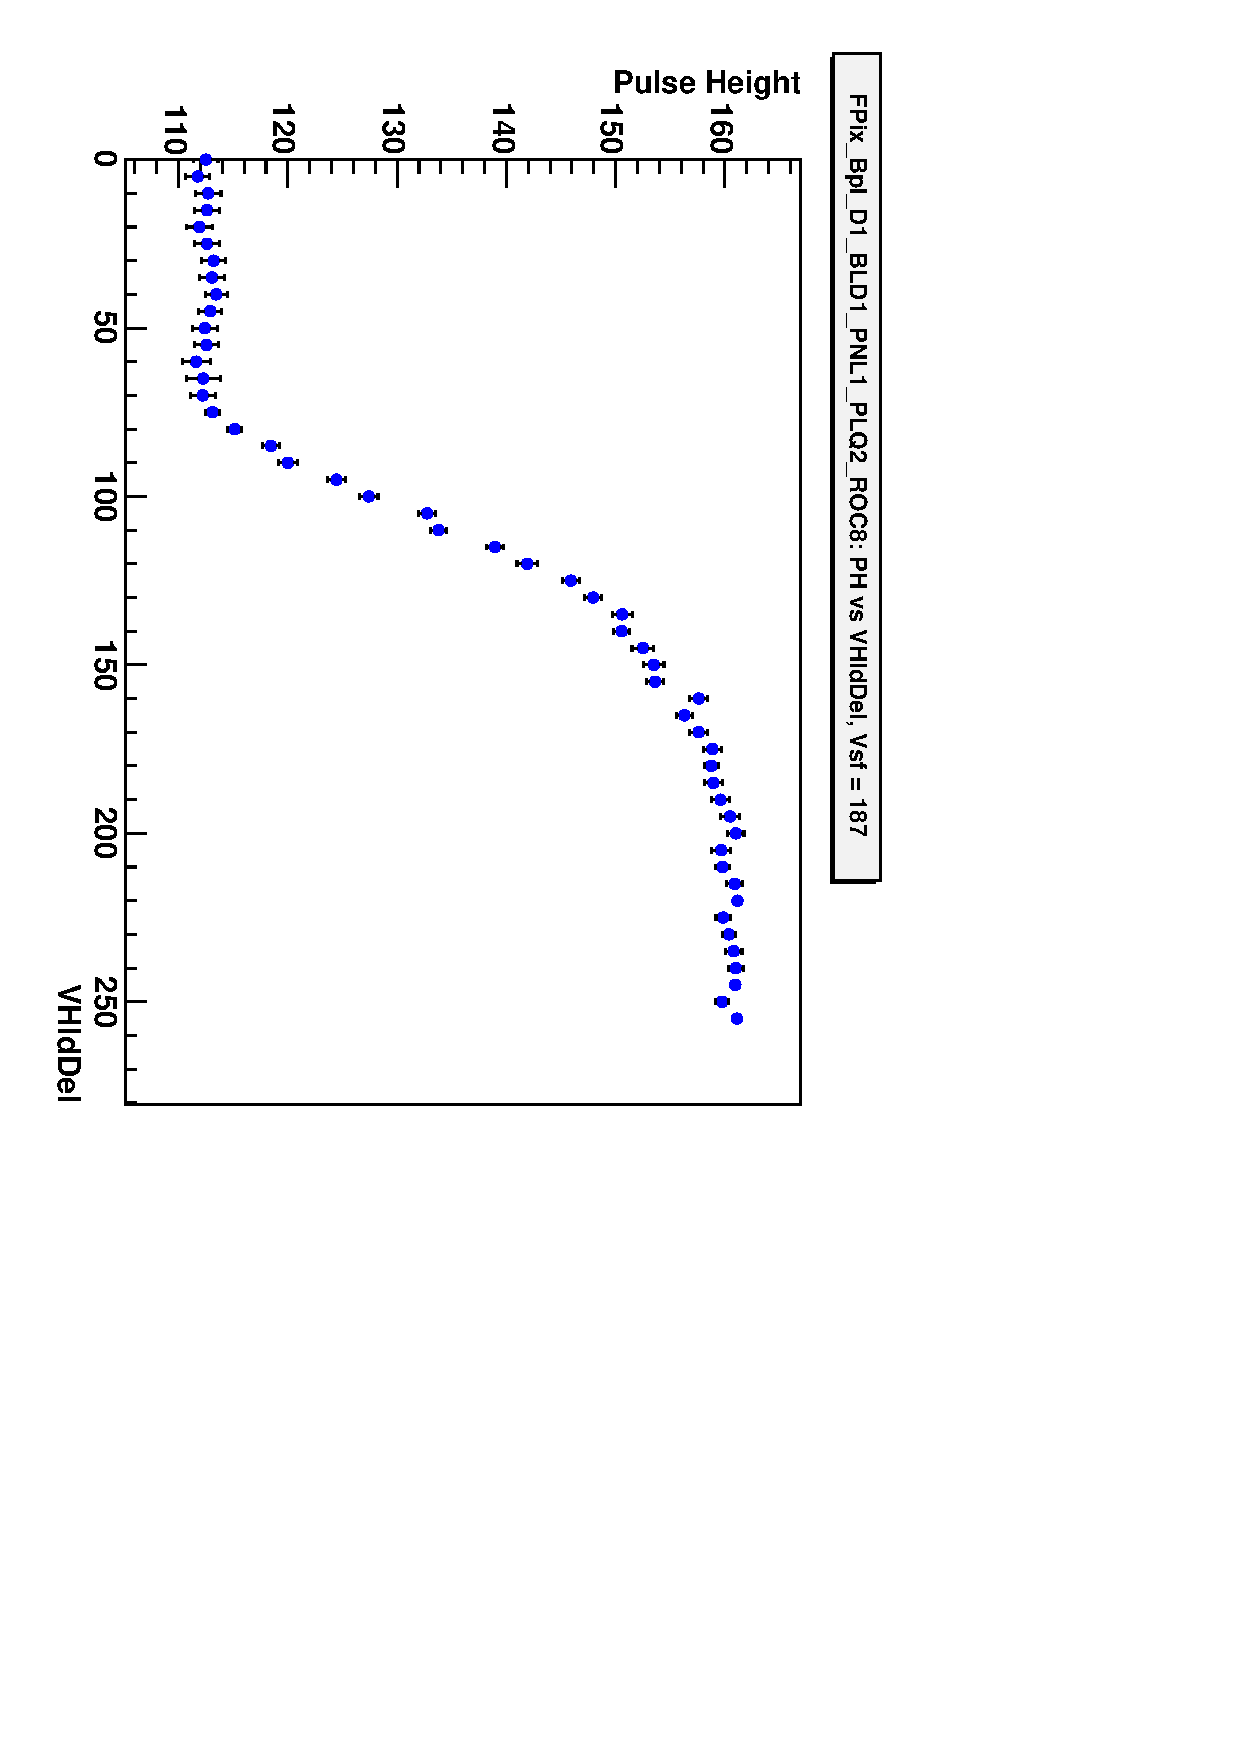
\includegraphics[angle=90,width=0.32\textwidth]{PH_vs_VHldDel_Vsf187.pdf}
 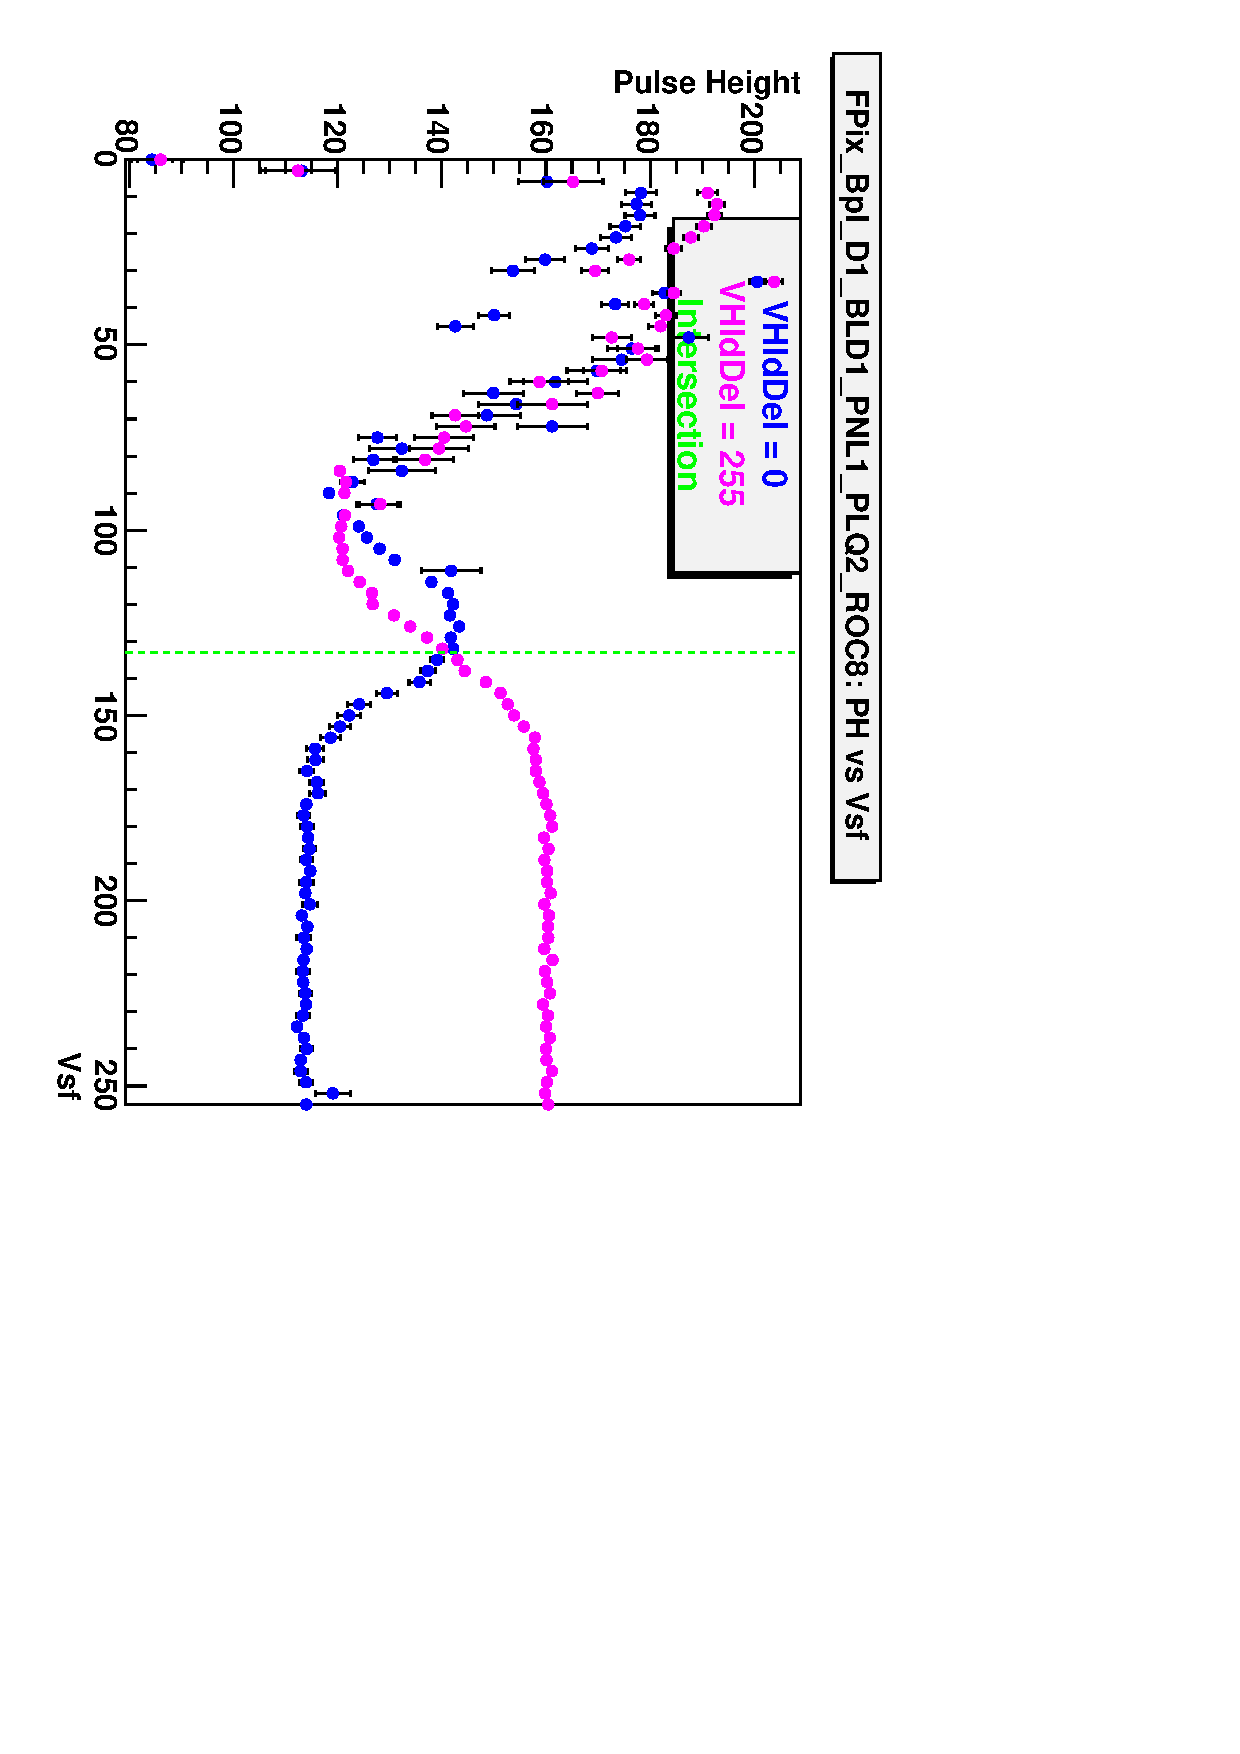
\includegraphics[angle=90,width=0.49\textwidth]{PH_vs_Vsf.pdf}
\end{center}
\caption{\emph{Top row:} Pulse height vs. VHldDel at low, medium, and high values of Vsf, with Vcal = 250 on the low scale.  As Vsf increases, the right endpoint increases.  The best Vsf value is the one for which the pulse heights measured at VHldDel = 0 and VHldDel = 255 are equal.  \emph{Bottom plot:} Pulse height at the endpoints of these plots, as a function of Vsf.  Low values of Vsf produce garbage output.}
\label{fig:PHvsVHldDel}
\end{figure}

After choosing a \verb|Vsf| value, \verb|VHldDel| should be set to the value that maximizes the pulse height.

When charge is injected with \verb|Vcal| = 250 on the low scale, these \verb|Vsf| and \verb|VHldDel| settings are found to give good linearity in pulse height vs.~injected charge, while not drawing too much power.

This procedure may be done in one calibration run, or it may be split into two -- the first to determine \verb|Vsf| and the second to determine \verb|VHldDel|.  Splitting into two runs is better because (1) it requires fewer scan points and (2) when the best \verb|Vsf| is a value interpolated between two scan points, the scan over \verb|VHldDel| will take place at that value instead of at the nearest \verb|Vsf| scan point.  The same calibration code can calibrate both DACs at once, or either one of them; calibration parameters determine which mode is used.  This is described in more detail below.

If the PSI algorithm described in Sec.~\ref{sec:LinearityVsVsf} is used to determine \verb|Vsf|, \verb|VHldDel| should be set with the algorithm used here -- maximizing pulse height at the chosen \verb|Vsf|.

\subsubsection{Vsf and VHldDel calibration steps}

This calibration consists of the following steps:
\begin{enumerate}
\item Scan \verb|Vsf| and \verb|VHldDel| according to the calibration's configuration.  On each trigger, read out data from each FED's FIFO3.  Record the pulse height.  If multiple pixels are enabled, average all of their pulse heights on each ROC.
\item If \verb|Vsf| was scanned, determine the best \verb|Vsf|.  To do this, make plots of pulse height vs.~\verb|Vsf| for the lowest \verb|VHldDel| scan value and for the highest \verb|VHldDel| scan value.  Take the rightmost intersection (the one at the largest \verb|Vsf|) as the best \verb|Vsf| value.  (When finding this intersection, interpolate between scan points.)  If the intersection point exceeds the maxVsf setting in the configuration for that ROC, reduce \verb|Vsf| to the maximum allowed.
\item If there are 3 or more \verb|VHldDel| scan points, determine the best \verb|VHldDel|.  If \verb|Vsf| was scanned, examine the scan of pulse height vs.~\verb|VHldDel| for the \verb|Vsf| scan point closest to the value chosen.  If \verb|Vsf| was not scanned, a scan of pulse height vs.~\verb|VHldDel| was taken at the \verb|Vsf| value stored in the configuration; examine this scan.  Find the scan point with the highest pulse height.  Calculate the parabola that passes through this point and the two adjacent points, and take the maximum of this parabola as the best \verb|VHldDel| value.  (If the highest point is an endpoint, use the endpoint as the best \verb|VHldDel|.)
\item Write out new ROC configuration files for the successfully-calibrated
ROCs with the new \verb|Vsf| and/or \verb|VHldDel| settings.
\item Print out a summary.
\end{enumerate}

\subsubsection{Parameters}
The standard parameters in \verb|calib.dat| may be used to control the
calibration.

The ``\verb|Repeat:|" parameter determines the number of triggers in each step
of the scan.  The ROC list is used to determine which ROCs are calibrated.

The hits specified in \verb|Rows:| and \verb|Columns:| will be
used.  At most two hits per pixel pattern may be specified (or alternatively SingleROC mode must be used); otherwise the calibration will abort.  The reason for this restriction is that the FED's spy FIFO3 will overflow if each ROC connected to it has more than two hits.

The scan ranges determine whether the calibration will determine only \verb|Vsf|, only \verb|VHldDel|, or both.  To determine just \verb|Vsf|, use something like:
\begin{verbatim}
VcalLow
Scan: Vsf     0 255 3    mix
Scan: VHldDel 0 255 255
Set:  Vcal 250
\end{verbatim}
This sets \verb|Vcal| = 250 on the low scale, just as Renaissance does.  The \verb|Vsf| scan is specified in the usual way.  The ``\verb|mix|'' flag must be enabled for \verb|Vsf| (or alternatively SingleROC mode must be used); otherwise the calibration will abort.  \verb|VHldDel| is also scanned, but with just two scan points -- the smallest and largest values.

To determine just \verb|VHldDel|, use something like:
\begin{verbatim}
VcalLow
Scan: VHldDel 0 255 5
Set:  Vcal 250
\end{verbatim}
\verb|Vsf| is not scanned, and a full scan is specified for \verb|VHldDel|.

To determine both \verb|Vsf| and \verb|VHldDel|, use something like:
\begin{verbatim}
VcalLow
Scan: Vsf     0 255 3    mix
Scan: VHldDel 0 255 5
Set:  Vcal 250
\end{verbatim}
Note that this scan is more time-consuming than running first for \verb|Vsf| and then for \verb|VHldDel|.  It also does not allow for the use of interpolated \verb|Vsf| values when determining \verb|VHldDel|.  Therefore, it is recommended to run two separate scans.

This calibration has no additional parameters aside from the standard ones.


\subsection{PHRange}

\subsubsection{Introduction and discussion}

A number of ROC DAC settings affect the scaling of the pulse height signal that is sent to the FED.  (This refers not to the actual charge collection, but to the translation of that charge into the signal sent out to the FED.)  We want the range of this signal -- the difference in recorded pulse height between small and large amounts of charge -- to be large.  However, the pulse height signal should not go low enough to be confused with the ultrablack level, nor high enough to exceed the FED's dynamic range.

The ROC DAC setting \verb|VIbias_PH| is intended to be used for adjusting the pulse height, so this DAC should be scanned.  Other DACs that affect the pulse height are \verb|VOffsetRO|, \verb|VIon|, and \verb|VOffsetOp|.  Previous studies found that adjusting \verb|VIbias_PH| and \verb|VOffsetOp|, while fixing \verb|VOffsetRO| and \verb|VIon|, worked well.~\cite{bib:Gromova}

\subsubsection{Pulse height calibration procedure}

The algorithm for this calibration is rather minimal.  In the configuration, the user specifies any number of arbitrary ROC DACs to be scanned, and also ``low" and ``high" amounts of injected charge (i.e. low and high \verb|Vcal| settings).  The pulse height is recorded at each scan point for the low and high charges.  (If multiple pixels are enabled, their pulse heights are averaged on each ROC.)  A scan point is discarded if either the low or high reading falls outside a user-specified range.  From the remaining scan points, the point chosen is the one with the largest pulse height difference between high and low charges.  These settings are written out.

If either 1 or 2 DACs are scanned, plots are generated of the high PH, low PH, and PH range (difference between high and low) as a function of the DAC setting(s).

\subsubsection{Parameters}

The standard parameters in \verb|calib.dat| may be used to control the calibration.

The ``\verb|Repeat:|" parameter determines the number of triggers in each step of the scan.  The ROC list is used to determine which ROCs are calibrated.

The hits specified in \verb|Rows:| and \verb|Columns:| will be used.  At most two hits per pixel pattern may be specified (or alternatively SingleROC mode must be used); otherwise the calibration will abort.  The reason for this restriction is that the FED's spy FIFO3 will overflow if each ROC connected to it has more than two hits.

The scan ranges are used to determine which DACs will be adjusted.  For example, to scan over \verb|VIbias_PH| and \verb|VOffsetOp|, use something like:
\begin{verbatim}
VcalHigh
Scan: VIbias_PH 0 255 5
Scan: VOffsetOp 0 255 5
Scan: Vcal 25 255 230
\end{verbatim}

Note that a \verb|Vcal| range should also be given.  The pulse height range at a given scan point will be calculated from the highest and lowest \verb|Vcal| for which hits were found.  If the final scan contains more than two \verb|Vcal| values with hits found, the points in the middle are ignored in determining the pulse height range.  Therefore, usual practice is to specify just two \verb|Vcal| scan points.  Note that if the lower \verb|Vcal| is below threshold, it will generate no hits; therefore the user should select a minimum that is above threshold.  If just one \verb|Vcal| value produces hits on a ROC, the calibration fails on that ROC.

Two optional parameters may also be set -- \verb|minPH| and \verb|maxPH|.  These specify the minimum and maximum allowable pulse height values; DAC settings that give pulse height outside of this range are rejected.  These parameters are specified on the scale of pulse height readings, which runs from 0 to 255.  This is in contrast to FED ADC counts, which run from 0 to 1023.  (Multiply the pulse height by 4 to get FED ADC counts.  For example, a PH of 75 corresponds to 300 FED ADC counts.)  These parameters default to 75 and 254; they may be changed in \verb|calib.dat|.  The parameters are summarized in Table~\ref{tab:PHRangeParameters}.

\begin{table}
\centering
\caption{Optional parameters for pulse height range calibration.}
\label{tab:PHRangeParameters}
\begin{tabular}{l@{~~~~}l@{~~~~}l}
\hline
\hline
Parameter & Default & Description \\
\hline
minPH                   &  75 = 300/4 & Minimum allowed pulse height \\
maxPH                   & 254         & Maximum allowed pulse height \\
\hline
\hline
\end{tabular}
\end{table}

\subsection{Vana and time walk}

{\it This calibration is not yet fully implemented. The description below represents what we intend to do.}

The idea is to run a scan of Vana vs CalDel. For a large charge we will assume that the response of different sensors is similar. As for a large charge (the maximum that can be injected) the raise time is small it is probably a reasonable assumption that we can assume that we have a small variation between ROCs. However, for a  smaller charge, like 250 on the low Vcal range, this is not obviously true. This calibration finds the time (absolute) that the Vcal=250 signal is over threshold and also finds the slope $dt/d{\rm Iana}$, or $dt/d{\rm Vana}$. Using this information the ROCs can be unified to one time at which a pulse of this strength passes over threshold.

%%%%%%%%%%%%%%%%%%%%%%%%%%%%%%%%%%%%%%%
%
% S E C T I O N   I N   P R O G R E S S 
%
%%%%%%%%%%%%%%%%%%%%%%%%%%%%%%%%%%%%%%%

\subsection{Trim bit determination}

{\it This section outlines an idea for triming. The actual
algorithms used are slightly different. The next section
describes the analysis tools that are available. This 
section should be updated.}

The algorithm described below is iterative. It uses a linerized
model to determine the parameters. Successive iterations of this
algorithm should provide better values of the trim parameters.

The threshold (for a pixel) is a function of Vcthr, Vtrim, and Trim.
\begin{equation}
{\rm Threshold}={\rm Threshold}({\rm pix}_i,{\rm Vcthr},{\rm Vtrim},
                {\rm Trim}_i)
\end{equation}
We can expand this as:

\begin{eqnarray*}
{\rm Threshold}({\rm pix}_i,{\rm Vcthr},{\rm Vtrim},{\rm Trim}_i)&=&
 {\rm Threshold}({\rm pix}_i,{\rm Vcthr}_0,{\rm Vtrim}_0,{{\rm Trim}_0}_i)\\
                    &+&{\rm deltaVcthr}{d{\rm Threshold}\over d{\rm Vcthr}}\\
                    &+&{\rm deltaVtrim}{d{\rm Threshold}\over d{\rm Vtrim}}\\
                    &+&{\rm deltaTrim}_i{d{\rm Threshold}\over d{\rm Trim}}
\end{eqnarray*}

Simplifying the notation we have

\begin{equation}
{\rm Threshold}({\rm pix}_i,{\rm Vcthr},{\rm Vtrim},{\rm Trim}_i)=
           A_i+B_i*{\rm deltaVcthr}+
           C_i*{\rm deltaVtrim}+
           D_i*{\rm deltaTrim}_i
\end{equation}

Now we want to set all of these equal to some value, {\rm ThrTrim}.

\begin{equation}
  {\rm ThrTrim}=A_i+B_i*{\rm deltaVcthr}+C_i*{\rm deltaVtrim}+
  D_i*{\rm deltaTrim}_i
\end{equation}

So we have $N$ equations and $N+2$ unknowns. Generally there are 
many solutions. But recall that the trim bits only takes on values
from 0 to 15. So we need more constraints. We use the following:

\begin{itemize}
\item We need to decide how many pixels we include in the triming.
      I.e. setting Vtrim large enough so that the trim bits can 
      adjust the threshold.
      Based on the 'initial' parameters find the rms of the threshold
      distribution. Find $n-\sigma$ and using an average $C_i$ 
      calculate deltaVtrim needed to include pixels out to $n-\sigma$.
      So this gives the first parameter. (Use $C_i$ for the smallest
      Vtrim.)


\item Require that the average trim is 7.5, that is
      $$ \sum_i {\rm deltaTrim}_i=\sum_i(7.5-{\rm Trim_i})$$
      This yields a simple constaint:
      $$
      {{\rm ThrTrim}\over D_i}={A_i \over D_i}+{B_i\over D_i}{\rm deltaVcthr}
      +{C_i\over D_i}{\rm deltaVtrim}+{\rm deltaTrim}_i
      $$
      and now summing over pixels give:
      $$\sum_i{{\rm ThrTrim \over D_i}}=
         \sum_i{A_i\over D_i}+\sum_i{B_i\over D_i}{\rm deltaVcthr}+
                     \sum_i{C_i\over D_i}{\rm deltaVtrim}+\sum_i(7.5-{\rm Trim_i})
      $$
      as we already have determined deltaVtrim we now also get 
      deltaVcthr.
\end{itemize}

Last all we have to do is to loop over all pixels and calculate deltaTrim$_i$.
This algorithm can be iterated to determined a better approximation of the trim bits.

The derivatives used above has to be determined numerically by running several Scurve runs. Need to describe how to do this; but this is really the core of the implementation.


\subsection{Trim bit analysis}

This section describes the tools that we have available today for trim bit determination.

\subsubsection{Running the threshold analysis}
\label{sect:analyzetrimrun}

The inputs to the threshold determination is Scurve runs with different parameters. After taking one of these Scurve runs it has to be analyzed to produce a file that contains the  thresholds for each pixel. 
After taking an SCurve (trim) run (TrimDefaultShort, TrimVcThrShort, TrimVtrimShort, TrimOnShort, TrimOffShort, TrimDefault, TrimVcThr, TrimVtrim, TrimOn, TrimOff) analyze the run using ./bin/linux/x86/PixelAnalysis.exe SCurve <runnum> 

The configuration/SCurveAnalysis.xml file needs to contain:
\begin{verbatim}
     <OutputTrimFile     Write="Yes"/>
\end{verbatim}
in order to generat the output needed in the trim analysis.

Currently this produces a very long output name.
Rename this file:
\begin{verbatim}
mv $POS_OUTPUT_DIRS/Run_100000/Run_100141/TrimOutputFile_Fed_32-33-34\
35-36-37-38-39.dat $POS_OUTPUT_DIRS/Run_100000/Run_100141/TrimDefault.dat
\end{verbatim}
For a 'TrimDefault' run.
For the other types of runs listed above they should be named:
\begin{verbatim}
TrimVcThr.dat
TrimVtrim.dat
TrimOn.dat
TrimOff.dat
\end{verbatim}

\subsubsection{Quality of trimming}
\label{sect:checktrims}

There is a command line tools that looks at the quality of the trimming. It can be run using:
\begin{verbatim}
[pixelpro@vmepcS2B18-17 test]$ ./bin/linux/x86/PixelTrimAnalysis.exe 100141 | more
Usage: PixelTrimAnalysis.exe runTrimDefault
trimDefault:/nfshome0/pixelpro/TriDAS_build7/pixel/PixelRun/Runs/Run_100000/\
Run_100141/TrimDefault.dat
All ROCs
FPix_BmO_D1_BLD1_PNL1_PLQ1_ROC0 81 64.1024 2.61066
FPix_BmO_D1_BLD1_PNL1_PLQ1_ROC1 81 69.239 1.39128
FPix_BmO_D1_BLD1_PNL1_PLQ2_ROC0 81 74.0942 1.6798
FPix_BmO_D1_BLD1_PNL1_PLQ2_ROC1 81 65.1567 1.36941
FPix_BmO_D1_BLD1_PNL1_PLQ2_ROC2 81 65.5652 1.4101
FPix_BmO_D1_BLD1_PNL1_PLQ2_ROC3 81 77.1227 2.36945
FPix_BmO_D1_BLD1_PNL1_PLQ2_ROC4 78 111.641 18.149
FPix_BmO_D1_BLD1_PNL1_PLQ2_ROC5 81 70.3416 1.4199
FPix_BmO_D1_BLD1_PNL1_PLQ3_ROC0 81 65.2256 1.4215
.
.
.
FPix_BpI_D2_BLD12_PNL2_PLQ3_ROC6 81 68.3048 1.82446
FPix_BpI_D2_BLD12_PNL2_PLQ3_ROC7 77 75.3988 1.54956
FPix_BpI_D2_BLD12_PNL2_PLQ3_ROC8 81 70.205 1.43413
FPix_BpI_D2_BLD12_PNL2_PLQ3_ROC9 81 59.5848 4.26486
Problem ROCs
FPix_BmO_D2_BLD1_PNL2_PLQ1_ROC3 81 49.3475 3.26693
FPix_BpO_D1_BLD9_PNL1_PLQ3_ROC2 11 65.2924 43.158
\end{verbatim}
Where the criteria for a problem ROC was set in the example above as a ROC with a threshold below 50 or with less than 50 hit pixels (out of 81). 
\subsubsection{Determining new VcThr settings}

If you just want to adjust VcThr to a fixed threshold you can run the following. First, take one 'TrimDefault(Short)' and one 'TrimVcThr(Short)'. In this example these are  runs 65624 and 65626 respectively. The 'TrimVcThr' run  adjusts VcThr (down) by a fixed amount for each ROC, e.g. 5 DAC settings. {\it Currently you have to manually make sure when you run the analysis below that this change of VcThr is conistent in the analysis program and in the configuration file. A relatively simple update in the future would be to automatically determine this change from the calib.dat files.} 
To run the analysis code 
\begin{verbatim}
./bin/linux/x86/PixelTrimVcThr.exe 10630 65624 65626 > log_TrimVcThr_65624
\end{verbatim}

10630 is the configuration key for run 65624. {\it Again this has to be manually supplied.} The output is a new set of dac settings in the current directory with new VcThr values. The target Vcal is set in {\tt src/common/PixelTrimVcThr.cc} on the line
\begin{verbatim}
    trimROC.setThrTrim(60.0);
\end{verbatim}
This is the target threshold in Vcal units.

The produced logfile is huge. One useful thing to do is:
\begin{verbatim}
grep deltaVcthr log_TrimVcThr_65624
\end{verbatim}
to see what the changes in VcThr are for the different ROCs.

\subsubsection{Make simple plots of thresholds}

To make simple plots of the thresholds do:

\begin{verbatim}
[pixelpro@vmepcS2B18-17 test]$ root -l
root [0] .L read.c
root [1] .x plot.c  
\end{verbatim}

plot.c specifies the input file.

\subsubsection{Full trim bit determination}
\label{sec:trimmingShort}
To do full trimming, i.e., adjusting the trim bits, Vtrim, and VcThr to trim the ROCs to a preset threshold the following steps are to be followed.

First you need to take five runs:
\begin{verbatim}
  TrimDefaultShort
  TrimVcThrShort
  TrimVtrimShort
  TrimOnShort
  TrimOffShort
\end{verbatim}
Normally, we use the 'short' configuration files that only use about 50 to 100 pixels on each ROC. This is enough pixels to find the  values need for VcThr and Vtrim on a given ROC. In a later step we  adjust just the trim bits for the remaining pixels. The TrimDefaultShort run is a run with the 'default' or current settings. The procedure is iterative and the parameters produced in this iteration will be the default parameters for the next iteration. The TrimVcThrShort and TrimVtrimShort runs adjusts the VcThr and Vtrim parameter by a default amount (typically -5 and +10 for VcThr and Vtrim respectively). The last two runs, TrimOnShort and TrimOffShort, turns the trim bits on and off respectively for each of the pixels. 
After taking these runs, they are analyzed as described in Sect.~\ref{sect:analyzetrimrun}. Having done this the new dac and trim bits are determined using
\begin{verbatim}
./bin/linux/x86/PixelTrim.exe <key> <runTrimDefault> <runTrimVcThr> \
<runTrimVtrim> <runTrimOn> <runTrimOff>
\end{verbatim}
Running this command produces new dac settings and trimbits. In addition if produces a file called 'rocder.dat'. The use of this file is described in the next section.

\subsubsection{Determining all trimbits}
\label{sec:trimbits}
Having carried out the procedure described in the previous section a file called 'rocder.dat' should have been produced. This file contains three numbers for each ROC determined from the analysis described above. First is the derivative of the threshold with respect to the VcThr setting. The second is the derivative of the threshold with respect to Vtrim {\it This needs to be defined more precisely.} The last is the change in the threshold with respect to changing trim bits, averaged over the pixels on the ROC. The change in threshold with respect to the  trimbits is used in the adjustment of the trim bits. 
A run is taken using the 'TrimDefault' configuration. This run is analyzed as described in Sect.~\ref{sect:analyzetrimrun}.
\begin{verbatim}
./bin/linux/x86/PixelTrimBits.exe <key> <runTrimDefault>
\end{verbatim}
Where {\tt <key>} is the global key used and {\tt <runTrimDefault>} is the run number for the trim default run. This produces new trim bit settings. The quality of the trimming can be checked as described in Sect.~\ref{sect:checktrims}.



